\chapter{Diseño e Implementación}

El proyecto tiene dos partes claramente diferenciadas a la hora de plantear el diseño:

\begin{itemize}
  \item \textbf{Diseño de clases.}
  \item \textbf{Diseño de las interfaces de usuario.}
  \item \textbf{Mecanismo de adición de vistas.}
\end{itemize}

Además, hay que tener en cuenta que uno de los objetivos principales es que la aplicación sea fácilmente extensible y que permita añadir nuevas interfaces de usuario para propiedades y dispositivos por lo que es parte importante de la fase de diseño, en la que se describirán todos detalladamente.

\bigskip
\section{Diseño de clases}

En todo proyecto de software es muy importante diseñar correctamente las clases antes de comenzar la fase de implementación. Un mal diseño puede provocar retrasos en la fase de implementación, incluso obligando a retroceder y rediseñarlas.

\bigskip
Podemos dividir el diseño en cuatro bloques:

\begin{itemize}
  \item \textbf{Diseño de las actividades de Android.}
  \item \textbf{Diseño del cliente INDI.}
  \item \textbf{Diseño de las clases manejadoras de propiedades.}
  \item \textbf{Diseño de las clases manejadoras de dispositivos.}
\end{itemize}

\newpage
\subsection{Diseño de las actividades de Android}

Las actividades en android son el cuerpo principal de las aplicaciones. Son ejecutadas en la hebra principal del sistema y gestionan la interfaz principal. Se pueden tener tantas actividades como se desee. En nuestro caso tenemos dos actividades:


\begin{itemize}
  \item \textbf{Front activity}
  \item \textbf{Main activity}
\end{itemize}

\subsubsection{Front activity}

Esta actividad inicia la aplicación, mostrando una pantalla de inicio con la información como portada. Una vez lanzada la aplicación esta actividad no volverá a ejecutarse a no ser que el sistema cierre la aplicación o que lo haga el usuario explícitamente. Como podemos ver en el diagrama de la figura \ref{fig:diag_front}, la actividad solo tiene una clase que hereda de \textit{AppCompatActivity}. Esta clase pertenece a la biblioteca de compatibilidad de \textbf{android}. Además, esta actividad tiene un objeto de la clase \textit{UpdateProgress}. Esta clase sirve para ejecutar código en una hebra separada en la que controlar el progreso.

\bigskip
\begin{figure}[!ht]
  \begin{center}
  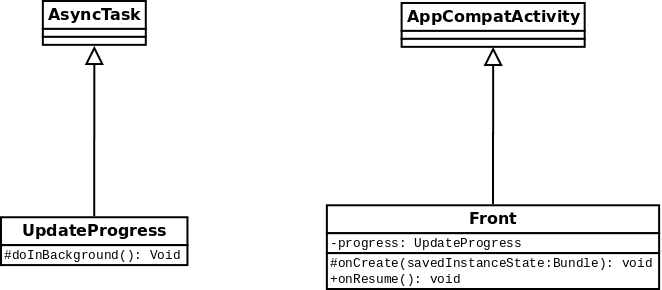
\includegraphics[width=1\textwidth]{../images/front_diag.png}
  \caption{Diagrama de clases de la actividad front}
  \label{fig:diag_front}
  \end{center}
\end{figure}


\subsubsection{Main activity}

La actividad principal es el núcleo de la aplicación. Esta clase es la más importante ya que su ciclo de vida condiciona el ciclo de vida de la aplicación. Es por ello que esta clase es la más compleja. En la figura \ref{fig:diag_main_activity} podemos ver el diagrama de clases. Las clases que no contienen ninguna especificación pertenecen a \textbf{Android} y simplemente se añaden para indicar las relaciones que las clases implementadas.

\bigskip
Dado que esta clase es la responsable de la visualización de los distintos menús, necesitamos declarar objetos de las clases que representan cada uno de los elementos visuales principales, tales como \textit{NavigationView}\cite{HTMMDND} o \textit{TabLayout}\cite{ATLWSV}.

\bigskip
Por otro lado, la actividad implementa una serie de escuchadores que le permiten capturar los eventos disparados por los distintos botones de la interfaz de usuario para realizar las acciones oportunas.

\bigskip
Además de estas clases, se ha diseñado la clase \textit{Settings} que representa las configuraciones generales de la aplicación: notificaciones y carpeta por defecto.

\bigskip
En el diagrama también podemos ver la clase \textit{Connection}. Esta clase representa las conexiones con el servidor y es por ella que se describen en el apartado correspondiente.


\bigskip
\begin{figure}[!ht]
  \begin{center}
  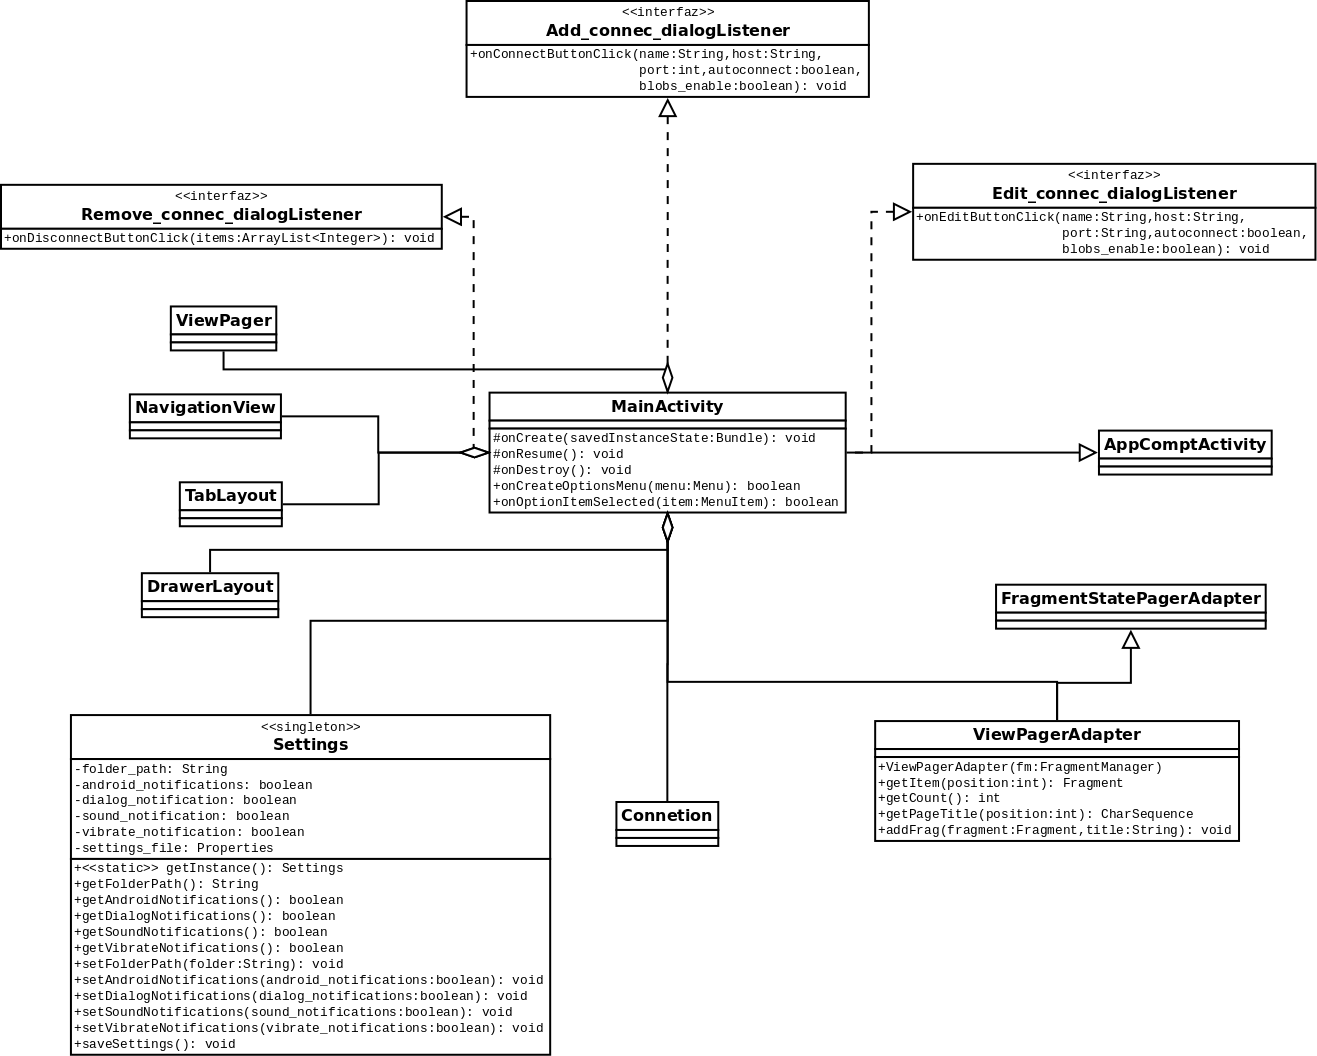
\includegraphics[width=1\textwidth]{../images/main_activity.png}
  \caption{Diagrama de clases de la actividad principal}
  \label{fig:diag_main_activity}
  \end{center}
\end{figure}


\newpage
\subsection{Diseño del cliente INDI}

La aplicación se basa en integrar la biblioteca \textbf{``INDI for Java''} para poder crear un cliente que nos permita conectarnos a cualquier servidor. Las conexiones se hacen creando conexiones TCP/IP a través de la red. \textbf{Android} establece unas restricciones muy fuertes respecto a la apertura y cierre de \textit{sockets} de red. Dado que la arquitectura del sistema esta basada en una única hebra principal que gestiona la interfaz de usuario, si iniciamos algún proceso que pueda bloquear dicha hebra, bloquearíamos todo el sistema. Por ello cualquier proceso de comunicación debe ejecutarse en una hebra secundaría. Además solo se pueden ejecutar acciones sobre la interfaz en la hebra principal.

\bigskip
Con estas restricciones, el primer paso necesario es extraer todo el código relativo a las conexiones a una hebra por conexión. Para ello se ha diseñado la clase \textit{Connection}. El objetivo principal de esta clase es lanzar en una hebra la apertura de la conexión y el intercambio de información con el servidor. Pero para poder utilizar esa información y mostrarla en pantalla necesitamos ejecutar en la hebra principal dichas acciones. 

\bigskip
\textbf{Android} nos facilita una clase para resolver este problema, aparentemente sin solución. La clase \textit{AsyncTask} tiene la peculiaridad de permitir ejecutar código en una hebra a parte y a la vez enviar información a la hebra principal para gestionarla adecuadamente. Por ello la clase \textit{Connection} lanza una hebra pero almacena en sus atributos el resultado de la conexión al servidor, permitiendo a la actividad principal procesar esos datos y mostrarlos adecuadamente. La actividad principal tendrá tantos objetos \textit{Connection} como conexiones se hayan añadido en la interfaz de usuario. Cada objeto \textit{Connection} creará una cliente INDI que le enviará todos los dispositivos y atributos que tenga y le irá informando de cualquier cambio para que estos se reflejen en la interfaz de usuario. Todas estas hebras se lanzan en paralelo, de forma que no ralenticen las acciones en la interfaz de usuario.

\bigskip
Por otra parte, para que todo funcione debemos diseñar una clase cliente \textbf{INDI} para crear la conexión, y escuchar cualquier cambio en propiedades, dispositivos o en la propia conexión. Por ello esta clase implementa las tres interfaces de \textbf{INDI}

\bigskip
Para facilitar el diseño, también se ha creado una clase \textit{device}. Esta clase se utiliza para procesar las propiedades de un dispositivo \textbf{INDI}. Cada propiedad pertenece a un grupo pero a priori no puedes conocer que grupos hay. Además las propiedades no llegan según un orden por lo que hay que comprobar por cada una a que grupo pertenece, si el grupo existe ya o si hay que crearlo. De la misma forma, cuando se borra una propiedad hay que comprobar si era la última de su grupo, en cuyo caso habrá que borrarlo. La clase \textit{device} facilita estas operaciones, añadiendo una capa de abstracción más para poder obtener las propiedades organizadas y listas para ser mostradas en la interfaz de usuario.

\bigskip
Finalmente, necesitamos representar la lista de propiedades y dispositivos. Para ello usamos las \textit{listas expandibles de Android}\cite{AELVT}. Estas listas nos permiten tener dos niveles. En el primer nivel mostramos los grupos y en el segundo los elementos. Internamente tenemos una lista o \textit{adaptador} de propiedades que añadimos a la clase \textit{PropertyArrayAdapter}. Cada objeto de esta clase representa un dispositivo con todas sus propiedades. 

\bigskip
En este punto cabe destacar que podemos tener propiedades ocultas. Dichas propiedades no deben ser añadidas al adaptador, ya que todos los elementos de este son mostrados. para controlarlo, la clase \textit{Connection} es la encargada de construir los \textit{adaptadores} a partir de la información del objeto de la clase \textit{IndiClient}. Por ello en la clase \textit{Connetion} gestionamos las propiedades que están ocultas para no agregarlas al \textit{adaptador} que le corresponda.


\bigskip
\begin{figure}[!ht]
  \begin{center}
  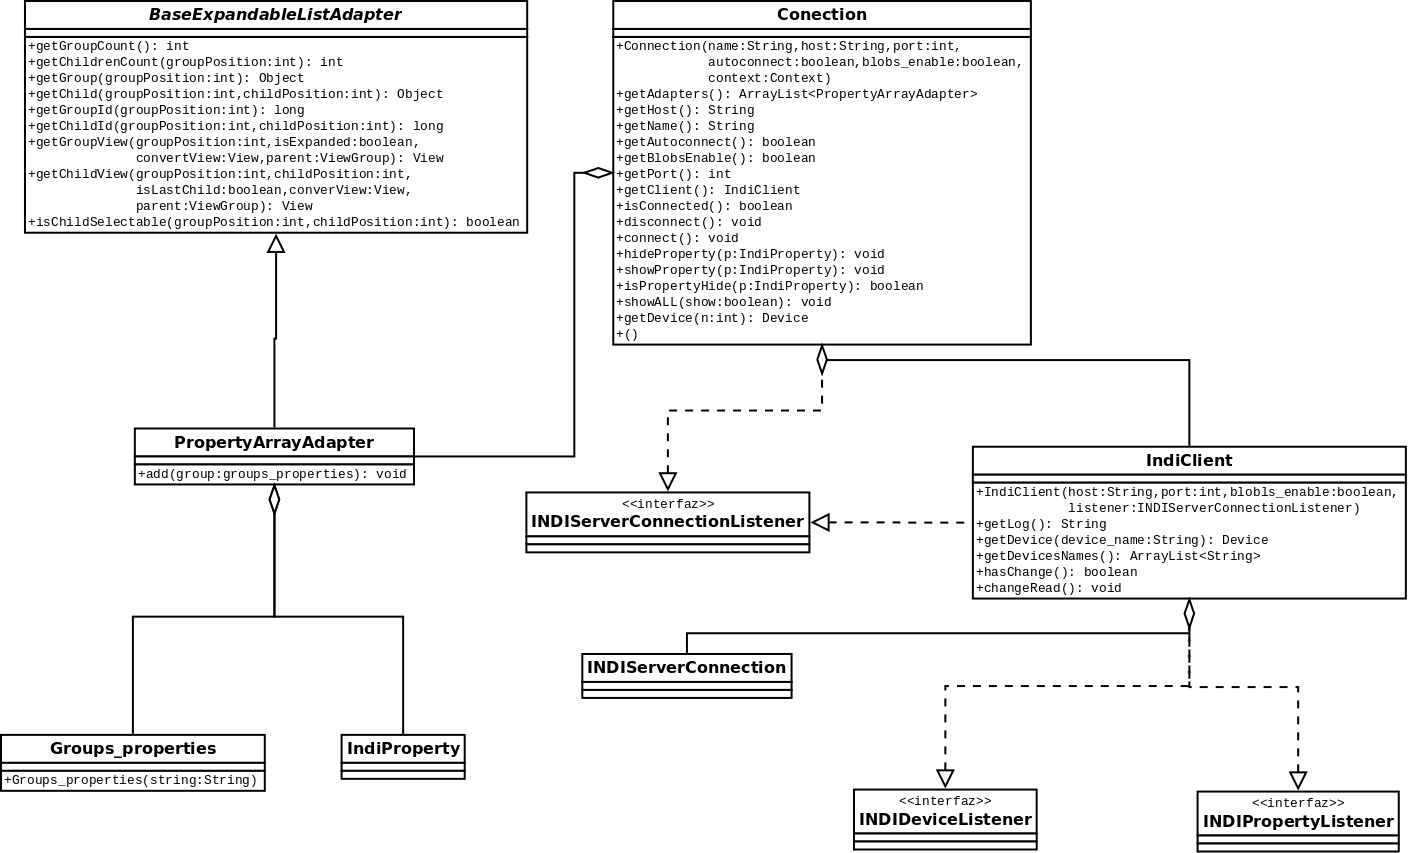
\includegraphics[width=1\textwidth]{../images/indi_diag_clases.png}
  \caption{Diagrama de clases asociadas a INDI}
  \label{fig:diag_indi_clases}
  \end{center}
\end{figure}


\newpage
\subsection{Diseño de las clases manejadoras de propiedades}

Como se explicó en la introducción, \textbf{INDI} maneja 5 tipos de propiedades:


\begin{itemize}
  \item \textbf{Text.}
  \item \textbf{Number.}
  \item \textbf{Switch.}
  \item \textbf{Blob.}
  \item \textbf{Light.}
\end{itemize}

\bigskip
Para manejar cada una de estas propiedades se crea una clase que recibirá un objeto \textit{INDIProperty} (del que heredan todos los tipos) y según el tipo informarán de que pueden manejar dicha propiedad y construirán las interfaces de usuario para mostrarla y editarla.

\bigskip
Gracias a la creación de la interfaz de Java \textit{UIPropertyManager} podemos añadir más manejadores de propiedades. Para ilustrar su uso se han creado dos manejadores más:

\begin{itemize}
  \item \textbf{Connection.}
  \item \textbf{Abort.}
\end{itemize}

\bigskip
Estas dos propiedades son de tipo \textit{Switch} pero tienen la peculiaridad de que siempre tienen la misma estructura: mismo número de elementos, mismo nombre para cada elemento, etc. Por ello podemos analizar la propiedad recibida y ver si es de esos tipos, informando de que podemos manejarla, y construyendo vistas especificas para esas propiedades (como son de tipo \textit{Switch} su vista por defecto sería la de todas las propiedades de este tipo).

\bigskip
En la figura \ref{fig:diag_manager_ui} podemos ver el diagrama de clases que ilustra la creación de los manejadores, implementando las interfaces para manejar propiedades y , adicionalmente, para manejar la pulsación sobre un objeto \textit{View} de Android.

\bigskip
\begin{figure}[!ht]
  \begin{center}
  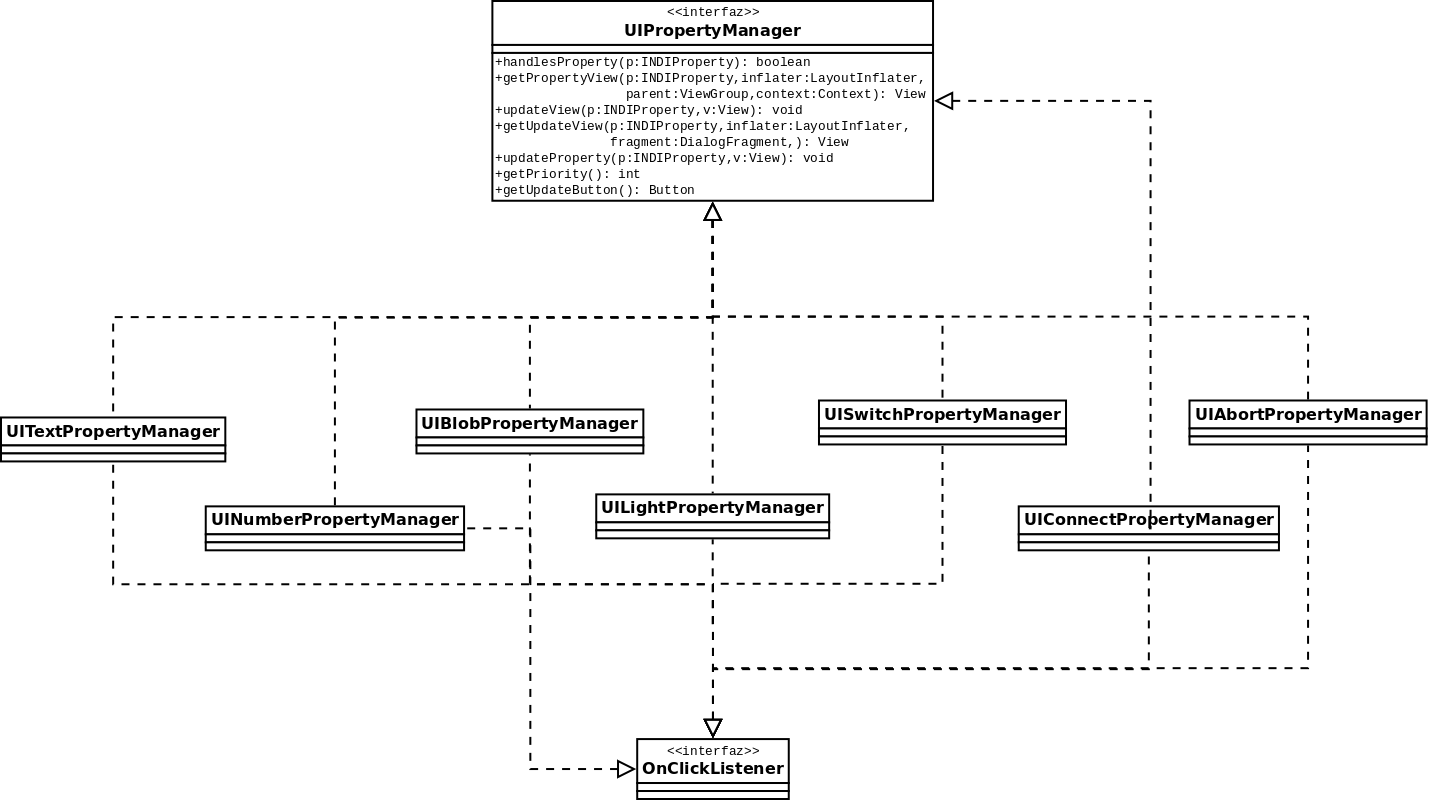
\includegraphics[width=1\textwidth]{../images/manager_ui.png}
  \caption{Diagrama de clases asociadas a los manejadores de propiedades}
  \label{fig:diag_manager_ui}
  \end{center}
\end{figure}

\newpage
\subsection{Diseño de las clases manejadoras de dispositivos}

Finalmente, necesitamos manejar y decidir como mostramos una propiedad y sus elementos. Para implementar esta funcionalidad se ha optado por utilizar los elementos visuales de Android \textit{tabs} que permiten mostrar vistas tabuladas. Con esto, vamos a crear una vista por defecto para cualquier dispositivo. Esta vista es la utilizada en las secciones anteriores: \textit{las listas expandibles de android}.

\bigskip
En la figura \ref{fig:diag_manager_ui_device} podemos ver que tenemos una clase \textit{DefaultDeviceView} que se mostrará por defecto para todas los dispositivos. Este es el comportamiento normal de la aplicación

\bigskip
Siguiente con el objetivo principal de facilitar la extensibilidad para añadir nuevas vistas de dispositivo, se ha diseñado una clase abstracta, \textit{DeviceView}, para facilitar la creación de nuevas vistas. Solo tenemos que crear una clase que herede de esta clase abstracta e implementar los métodos. Al ser una clase que hereda de \textit{Fragment}, dentro de ella tenemos libertad para mostrar las propiedades del dispositivo para personalizarlo. Cada nueva vista sería una tabulación más en la vista tabulada.


\bigskip
\begin{figure}[!ht]
  \begin{center}
  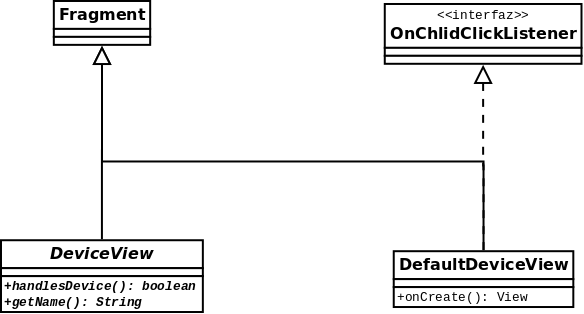
\includegraphics[width=1\textwidth]{../images/device_ui.png}
  \caption{Diagrama de clases asociadas a los manejadores de dispositivos}
  \label{fig:diag_manager_ui_device}
  \end{center}
\end{figure}


\bigskip
\section{Diseño de las interfaces de usuario}

Las interfaces de usuario deben ser objeto de un cuidadoso diseño dado que estamos construyendo una aplicación móvil, y el éxito dependerá en gran medida de una buena interfaz de usuario que sea útil, clara y fácil de usar.

\bigskip
A lo largo del diseño de las interfaces de usuario, se fueron mejorando sucesivamente las distintas vistas desde bocetos en papel (figuras \ref{fig:boceto} y \ref{fig:boceto_2}) hasta primeras versiones ya implementadas en la aplicación (figuras \ref{fig:capturas} y \ref{fig:capturas2}).


\begin{figure}
    \centering
    \begin{subfigure}[]{0.4\textwidth}
        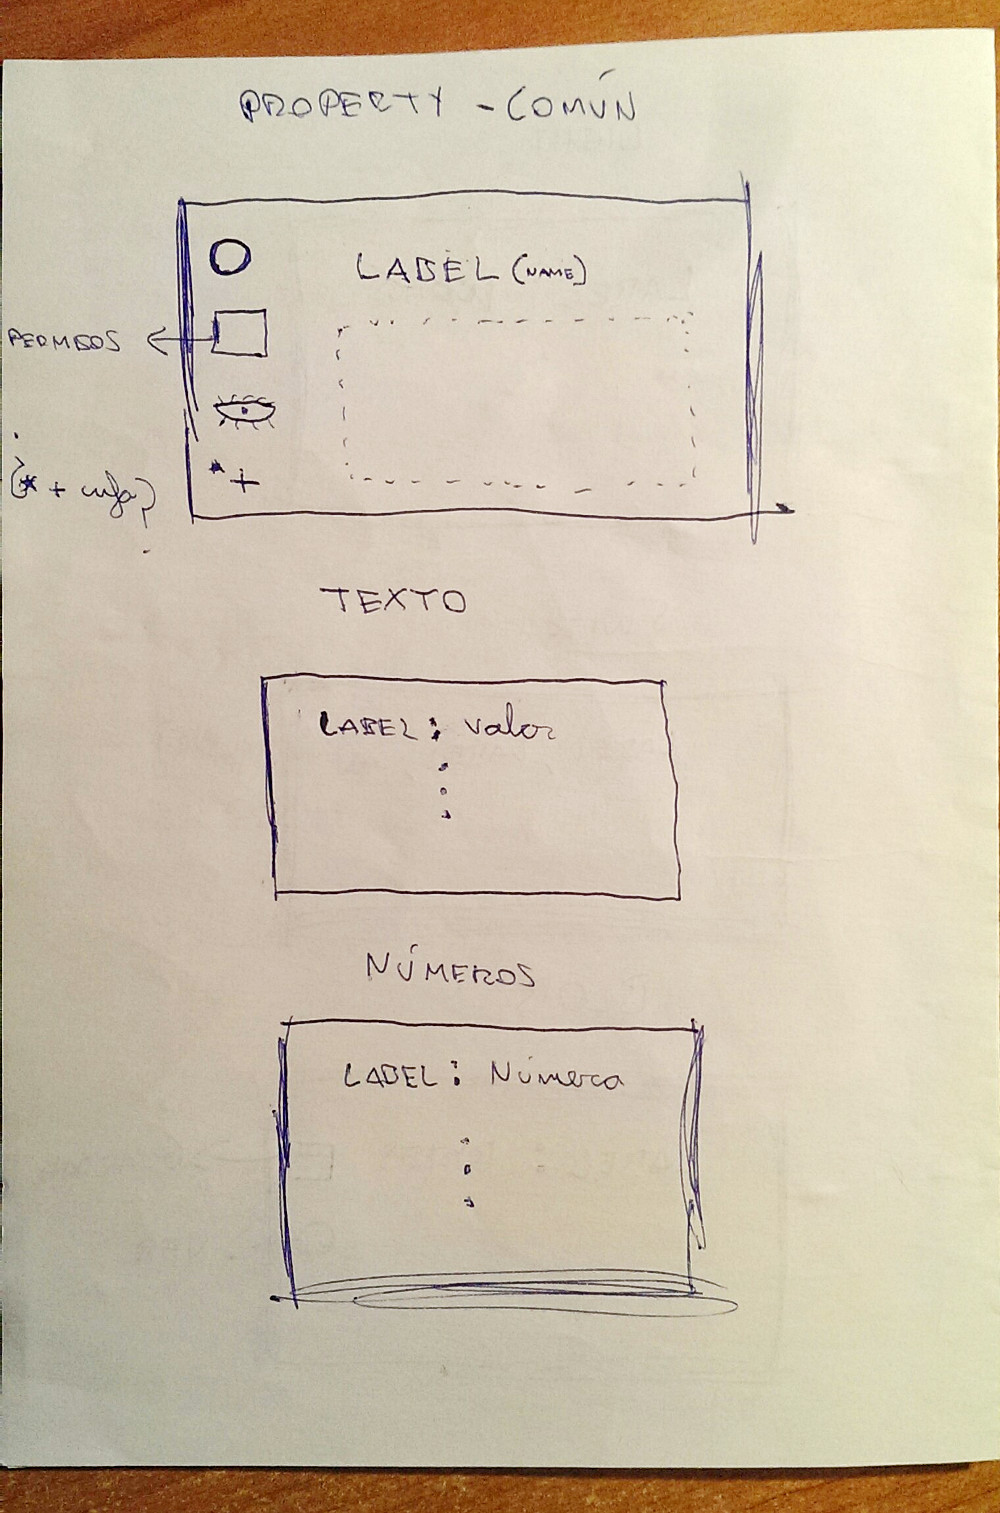
\includegraphics[width=\textwidth]{../images/boceto.jpg}
        \caption{}
        \label{fig:boceto}
    \end{subfigure}
    \begin{subfigure}[]{0.4\textwidth}
        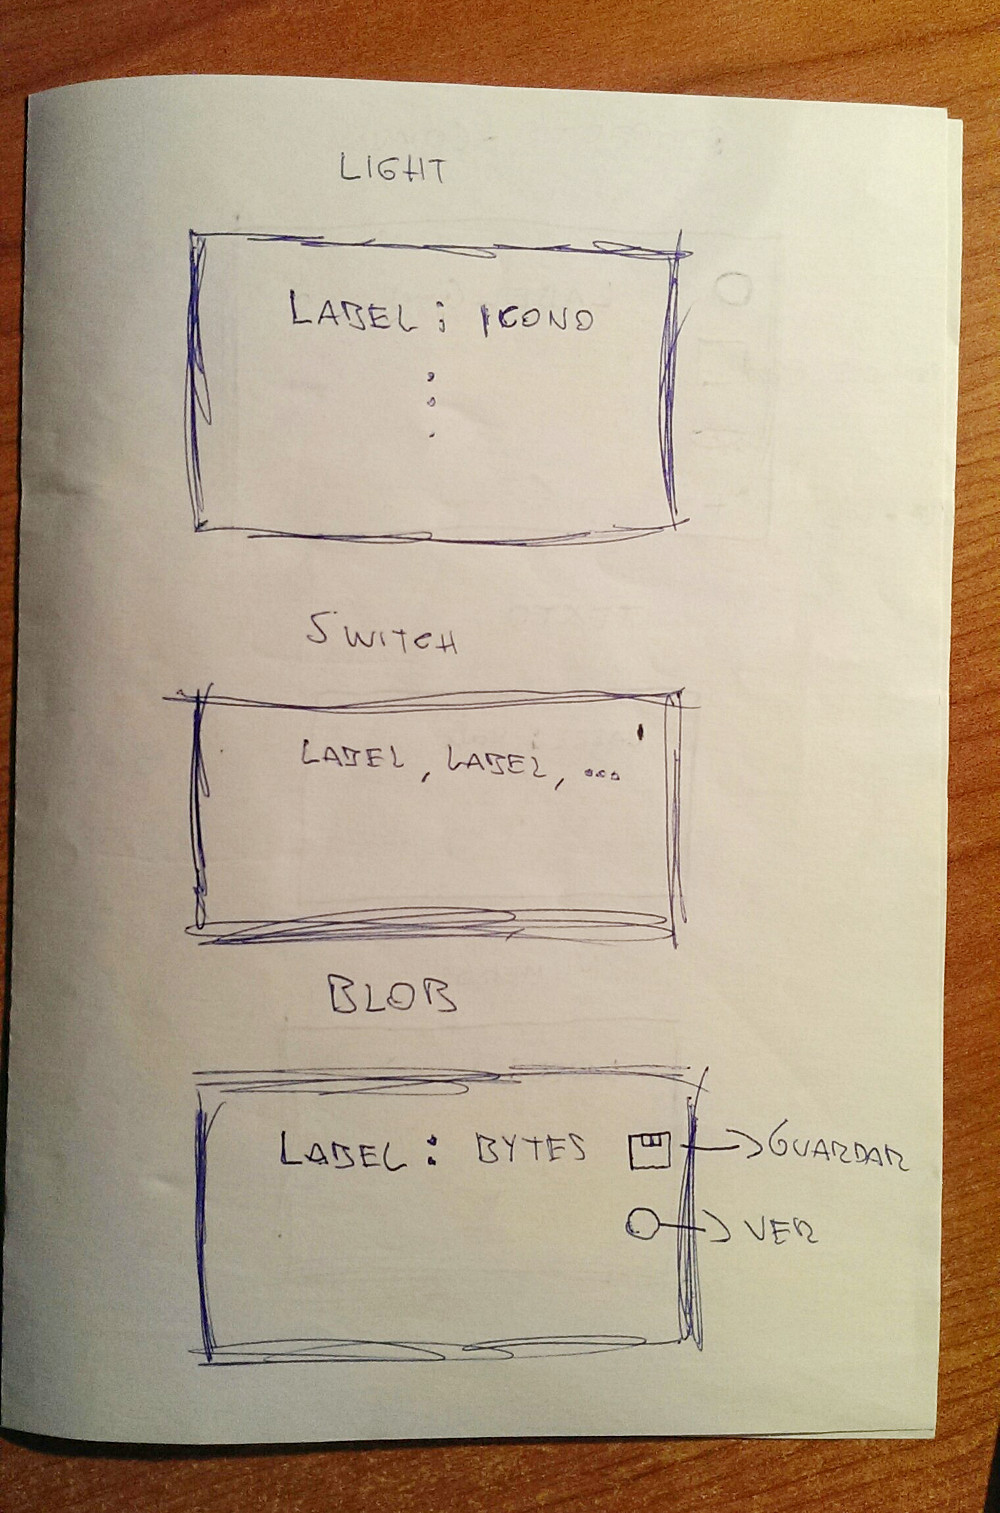
\includegraphics[width=\textwidth]{../images/boceto2.jpg}
        \caption{}
        \label{fig:boceto_2}
    \end{subfigure}
    \caption{Bocetos}\label{fig:bocetos}
\end{figure}

\begin{figure}
    \centering
    \begin{subfigure}[]{0.4\textwidth}
        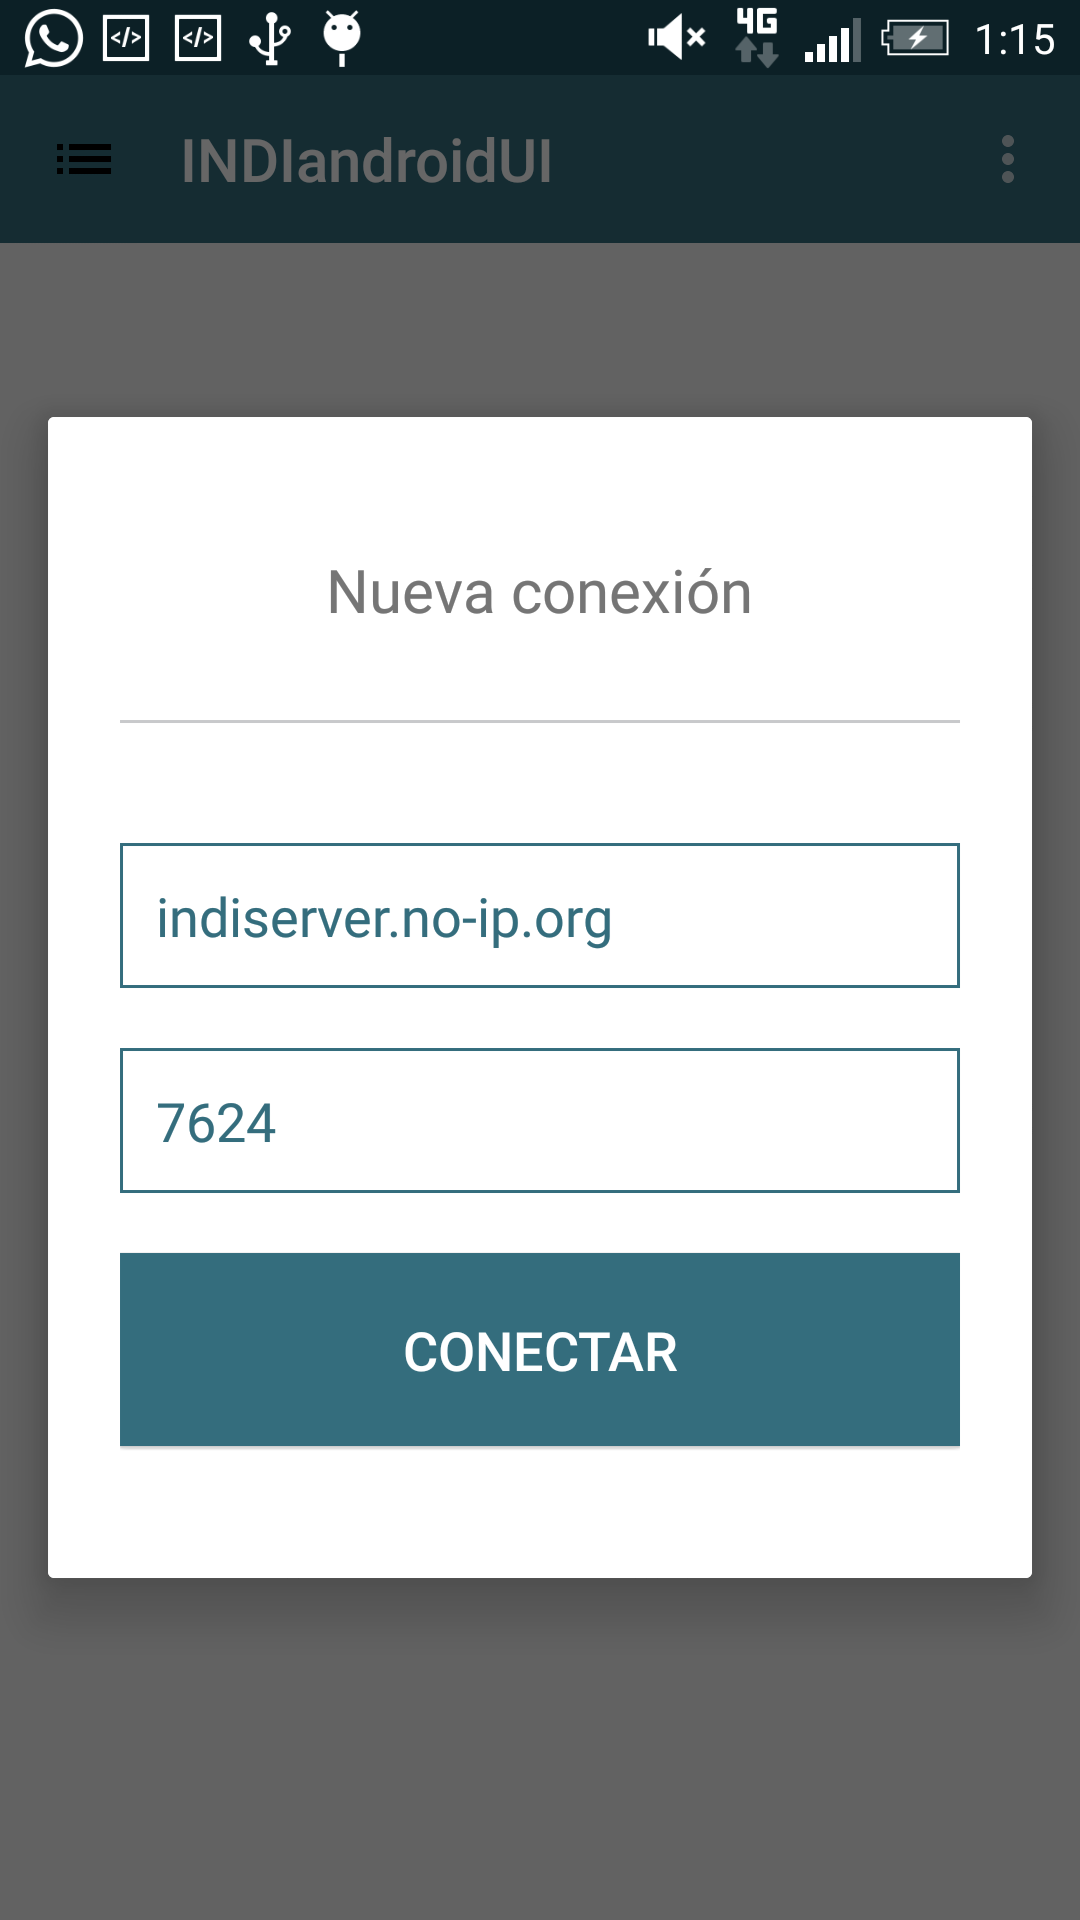
\includegraphics[width=\textwidth]{../images/captura.png}
        \caption{}
        \label{fig:captura1}
    \end{subfigure}
    \begin{subfigure}[]{0.4\textwidth}
        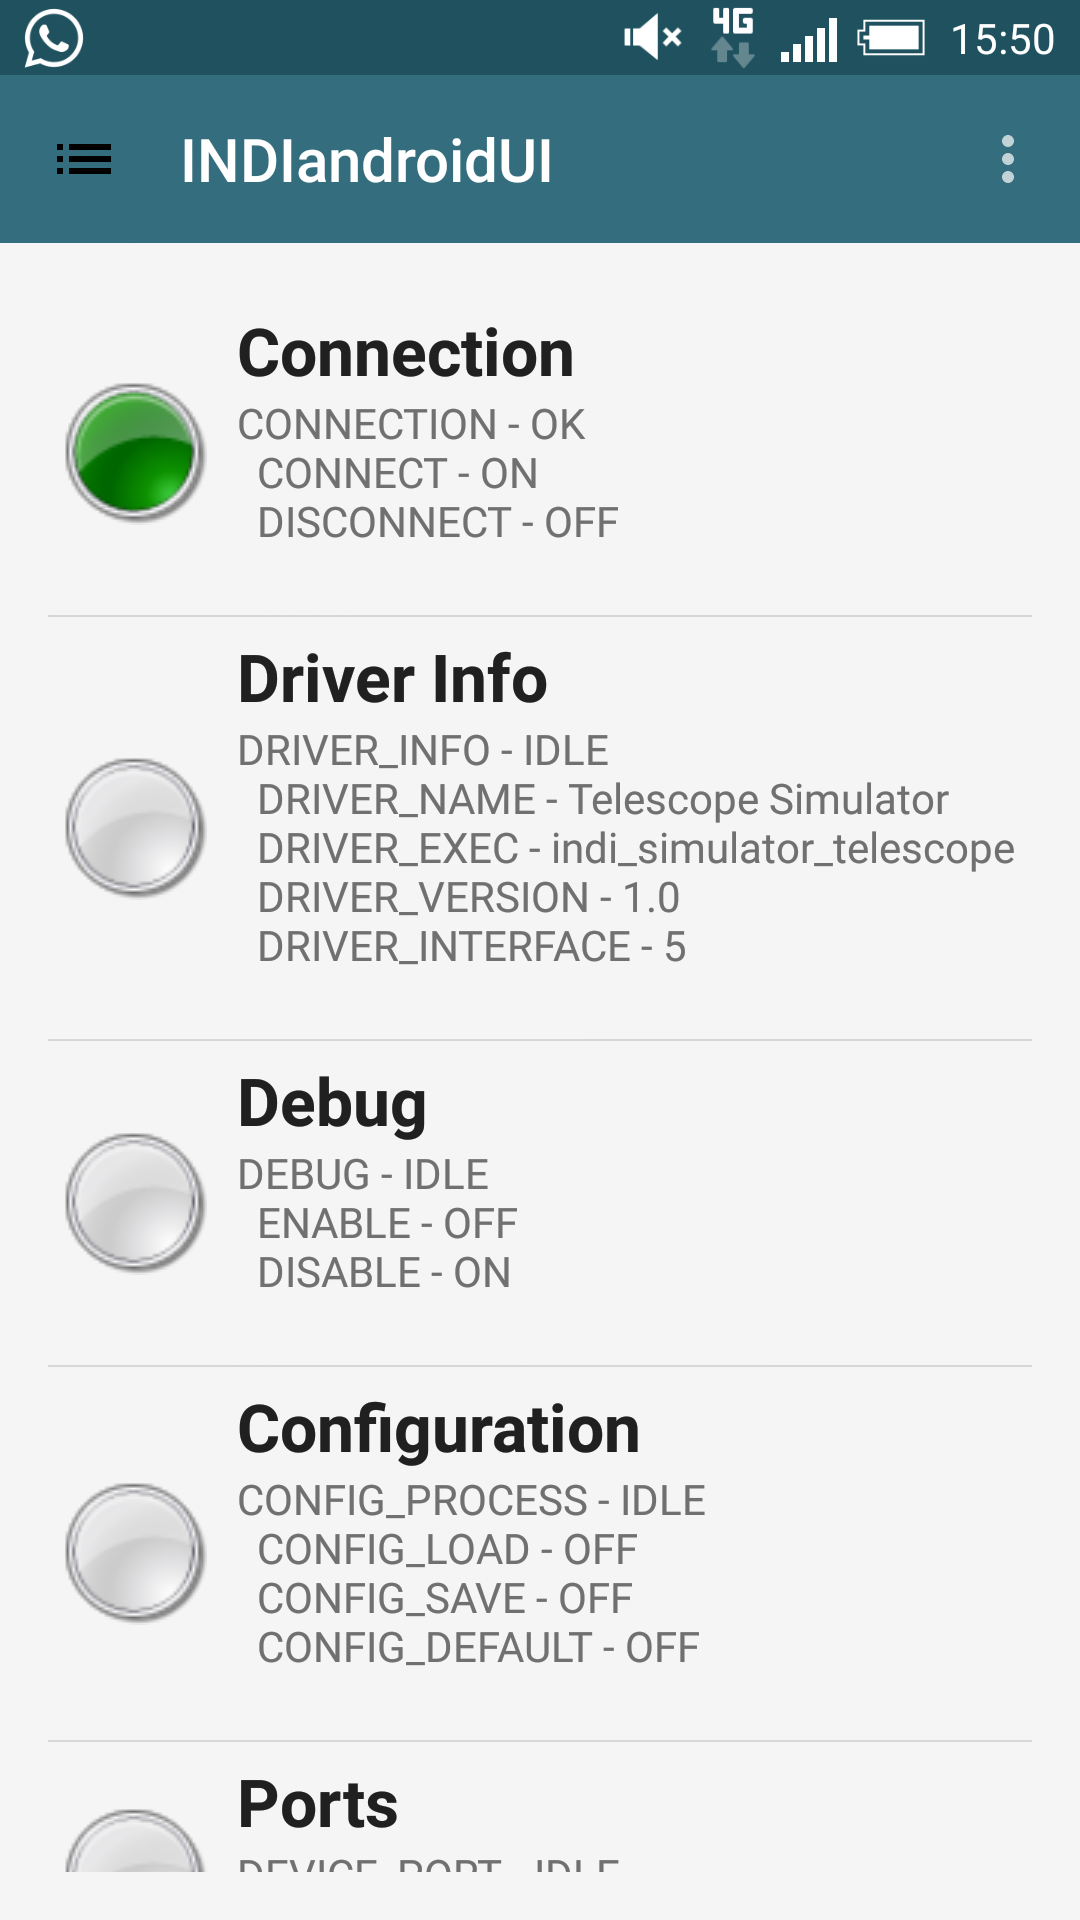
\includegraphics[width=\textwidth]{../images/captura2.png}
        \caption{}
        \label{fig:captura2}
    \end{subfigure}
    \caption{Capturas}\label{fig:capturas}
\end{figure}

\begin{figure}
    \centering
    \begin{subfigure}[]{0.4\textwidth}
        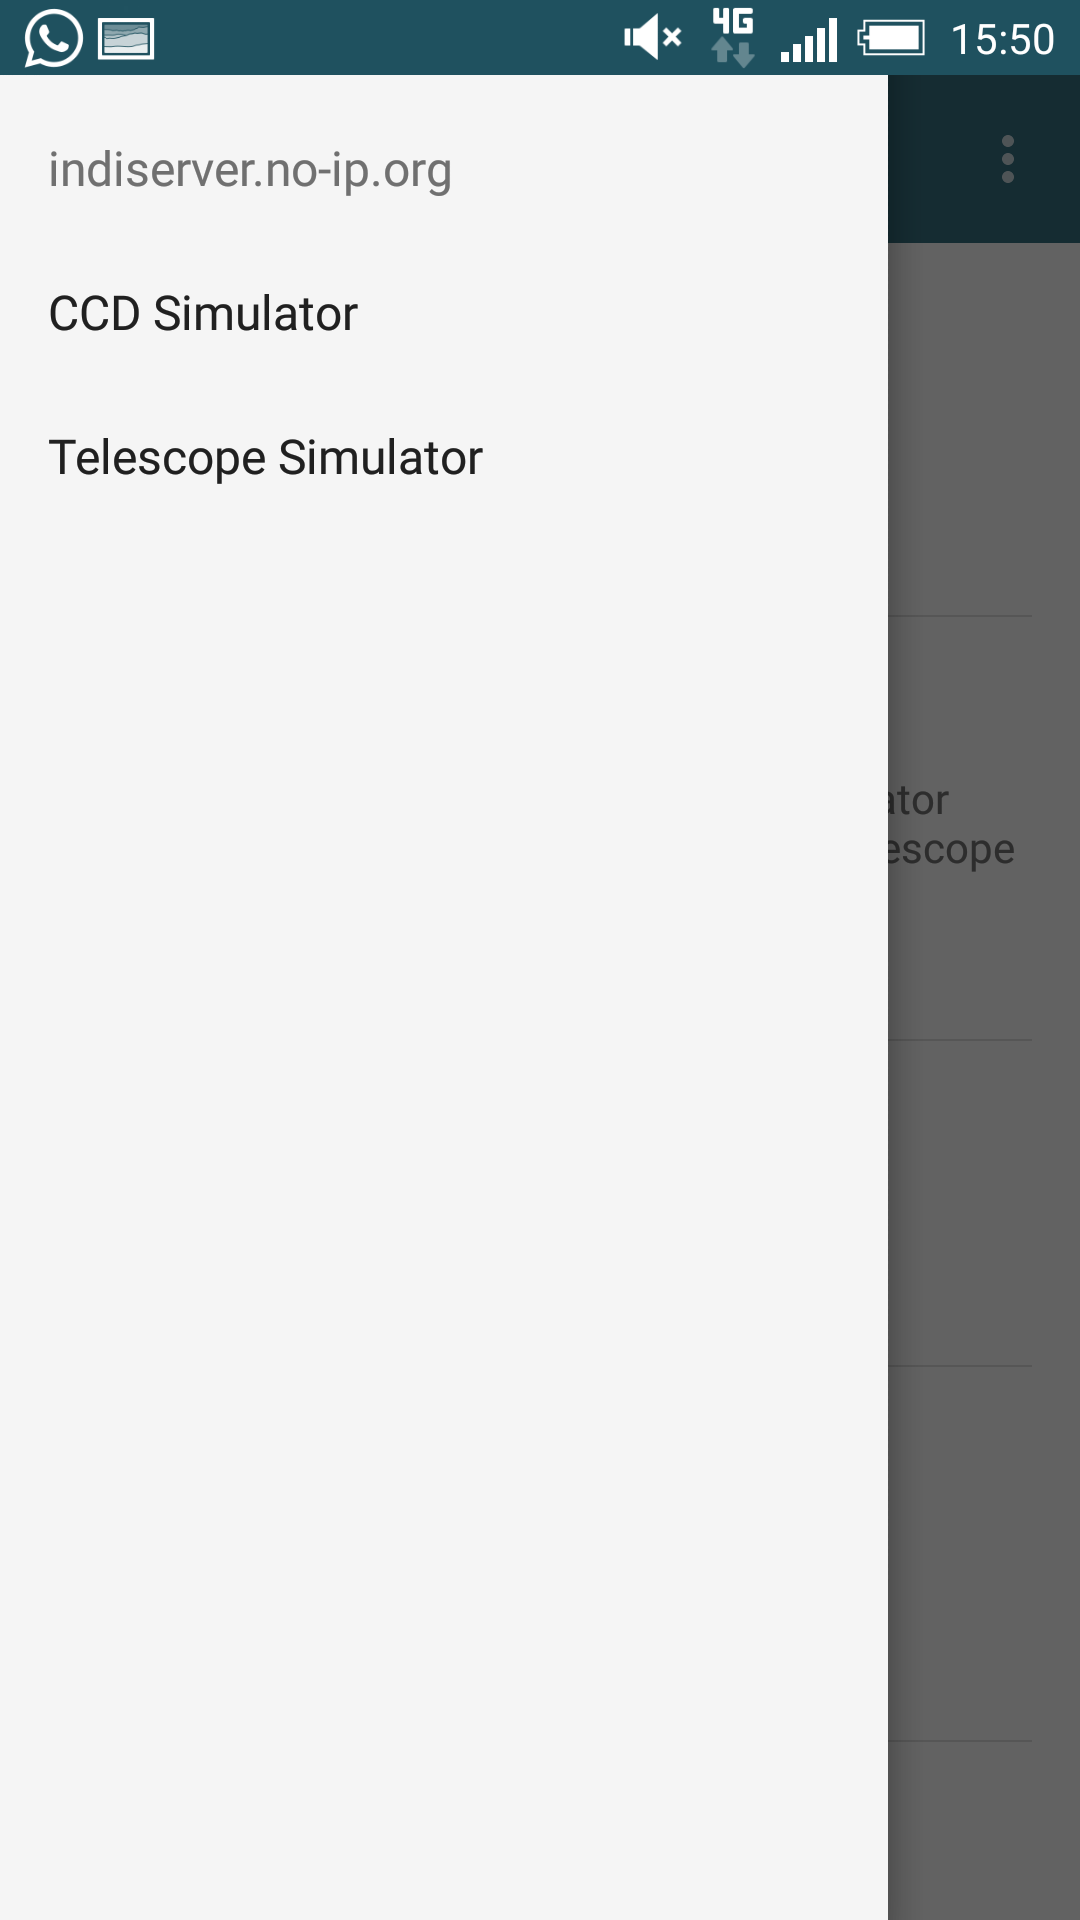
\includegraphics[width=\textwidth]{../images/captura3.png}
        \caption{}
        \label{fig:captura3}
    \end{subfigure}
    \begin{subfigure}[]{0.4\textwidth}
        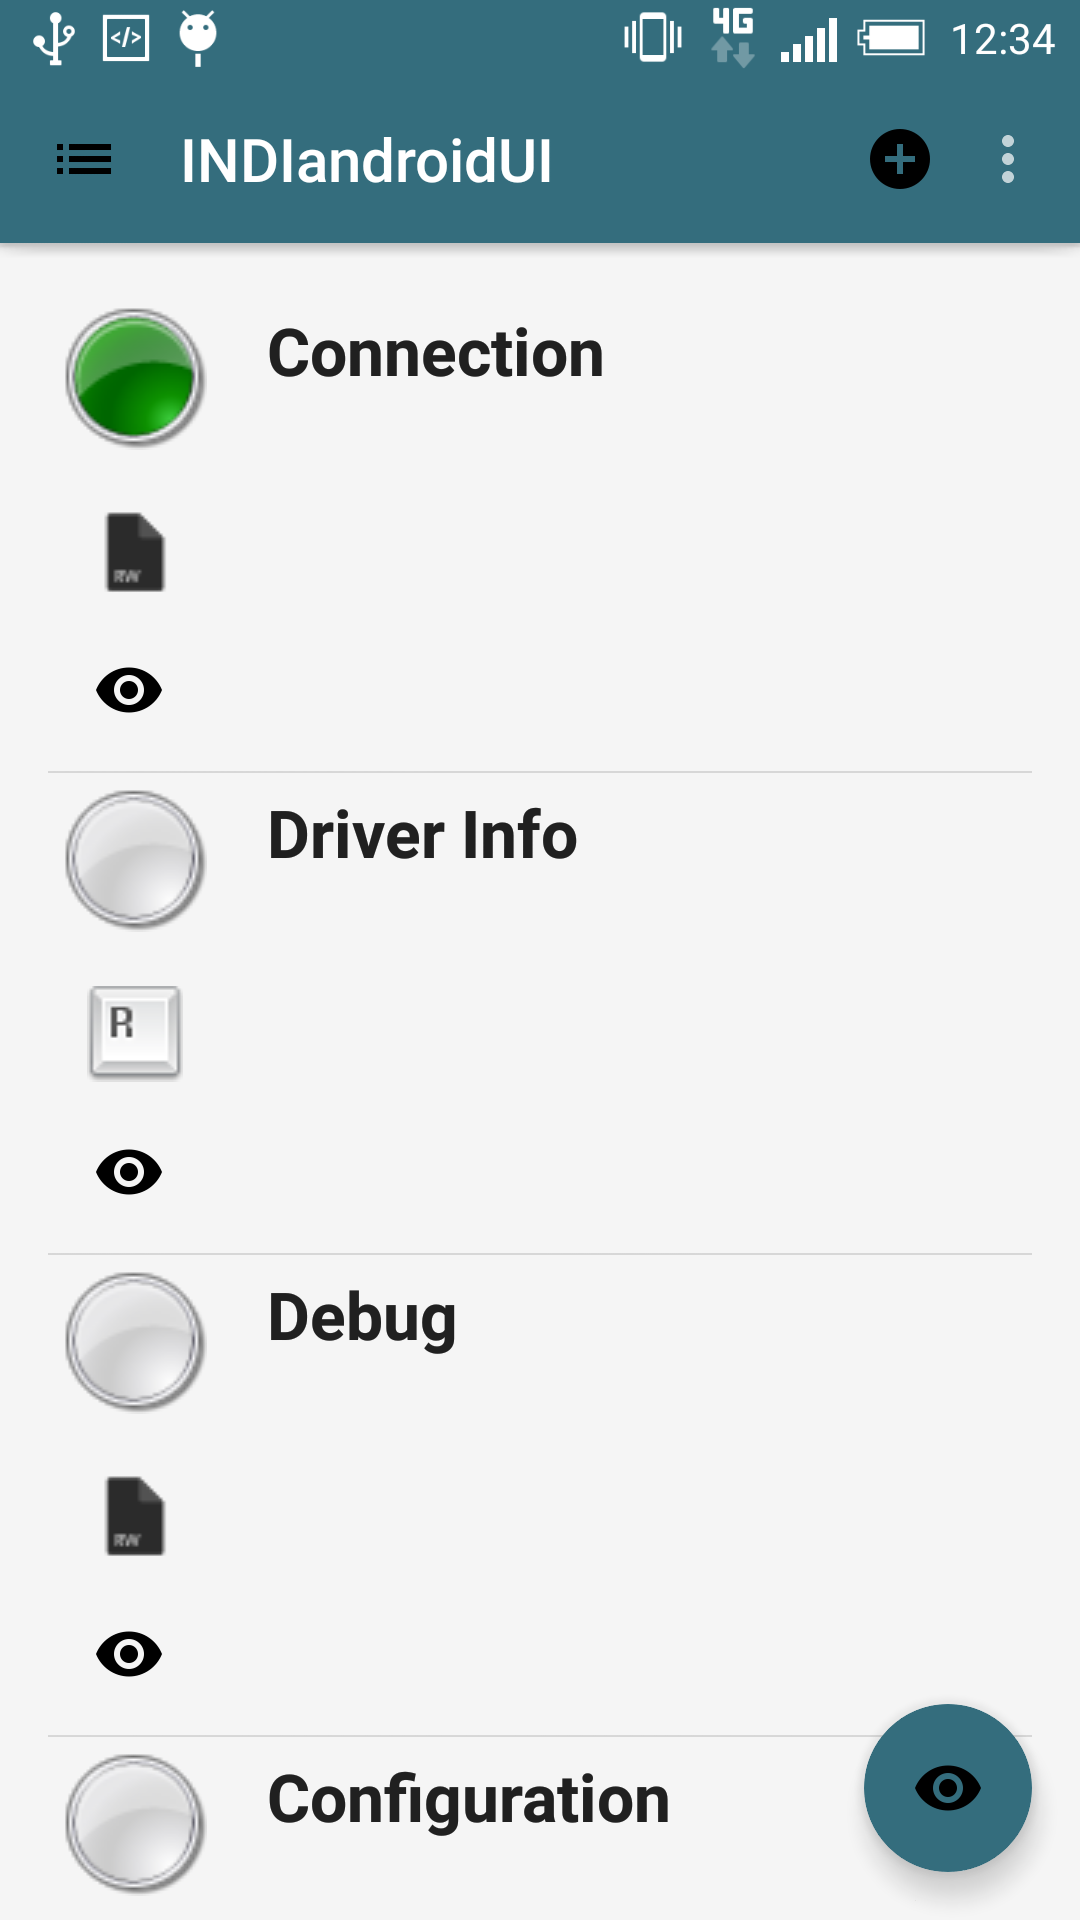
\includegraphics[width=\textwidth]{../images/captura5.png}
        \caption{}
        \label{fig:captura4}
    \end{subfigure}
    \caption{Capturas}\label{fig:capturas2}
\end{figure}

\bigskip
En cada una de las iteraciones del proceso \textbf{Scrum} se fueron rediseñando y mejorando las interfaces de usuario hasta llega a las vistas finales descritas en los siguientes apartados.

\bigskip
Para poder abordar mejor el diseño, se han separados las interfaces en los siguientes grupos:

\begin{itemize}
  \item \textbf{Interfaz principal de la aplicación.}
  \item \textbf{Interfaz para listar las propiedades.}
  \item \textbf{Interfaz de propiedad.}
  \item \textbf{Interfaz de diálogos}
  \item \textbf{Interfaz del log}
  \item \textbf{Interfaz de los ajustes}
\end{itemize}

\bigskip
\subsection{Interfaz principal de la aplicación}

La interfaz principal es la más importante de cara al usuario. Define como se va a organizar toda la información y la navegabilidad dentro de la aplicación. 

\bigskip
En cada iteración se han añadido nuevas funcionalidades a la aplicación lo cual provocaba tener que definir aspectos de la interfaz de usuario principal. 

\bigskip
Por otro lado, en un esfuerzo por seguir las directrices de \textbf{Android} y las tendencias actuales en las aplicaciones móviles, se han incorporado los elementos más actuales tales como la barra de navegación lateral con estilo \textit{material desing} o tener vistas tabuladas. En las figuras \ref{fig:capturas3} y \ref{fig:capturas4} podemos ver la interfaz principal de la aplicación.

\begin{figure}
    \centering
    \begin{subfigure}[]{0.4\textwidth}
        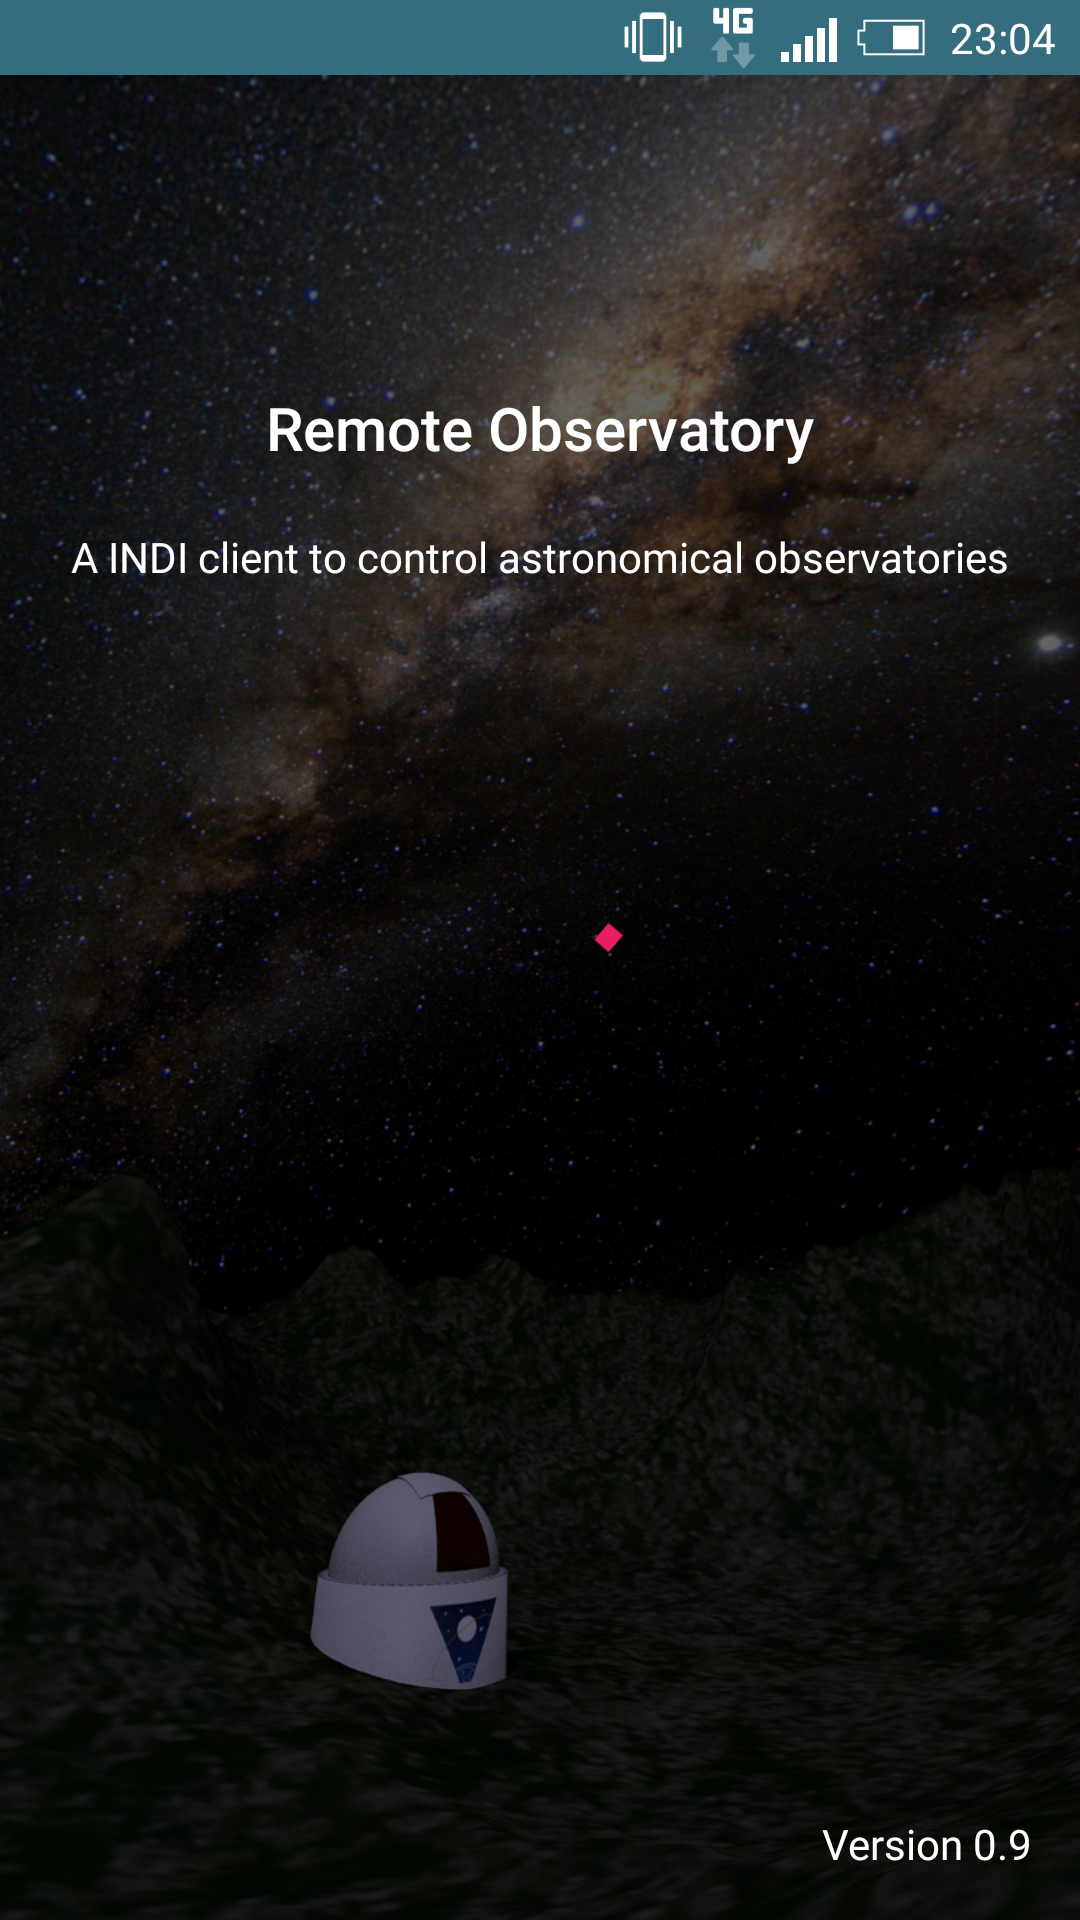
\includegraphics[width=\textwidth]{../images/captura6.png}
        \caption{}
        \label{fig:captura4}
    \end{subfigure}
    \begin{subfigure}[]{0.4\textwidth}
        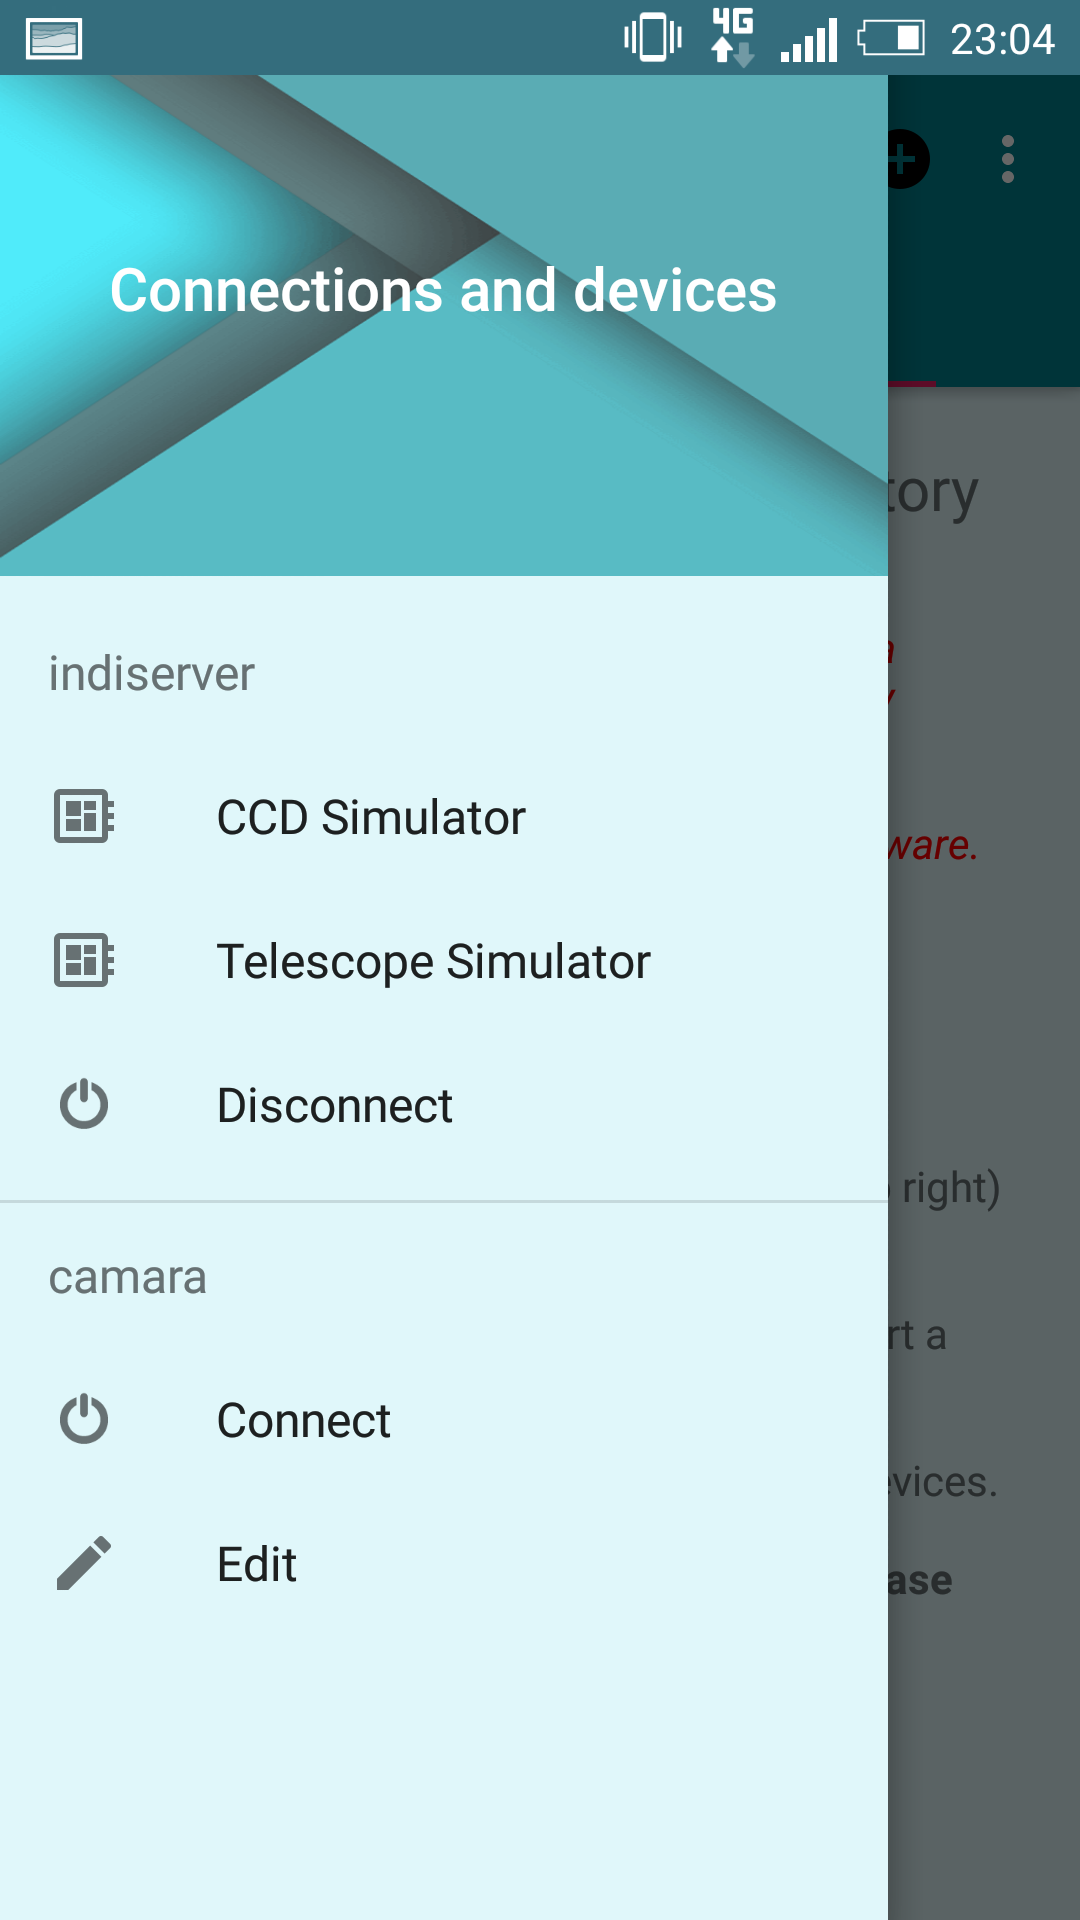
\includegraphics[width=\textwidth]{../images/captura7.png}
        \caption{}
        \label{fig:captura5}
    \end{subfigure}
    \caption{Capturas de la interfaz principal}\label{fig:capturas3}
\end{figure}

\begin{figure}
    \centering
    \begin{subfigure}[]{0.4\textwidth}
        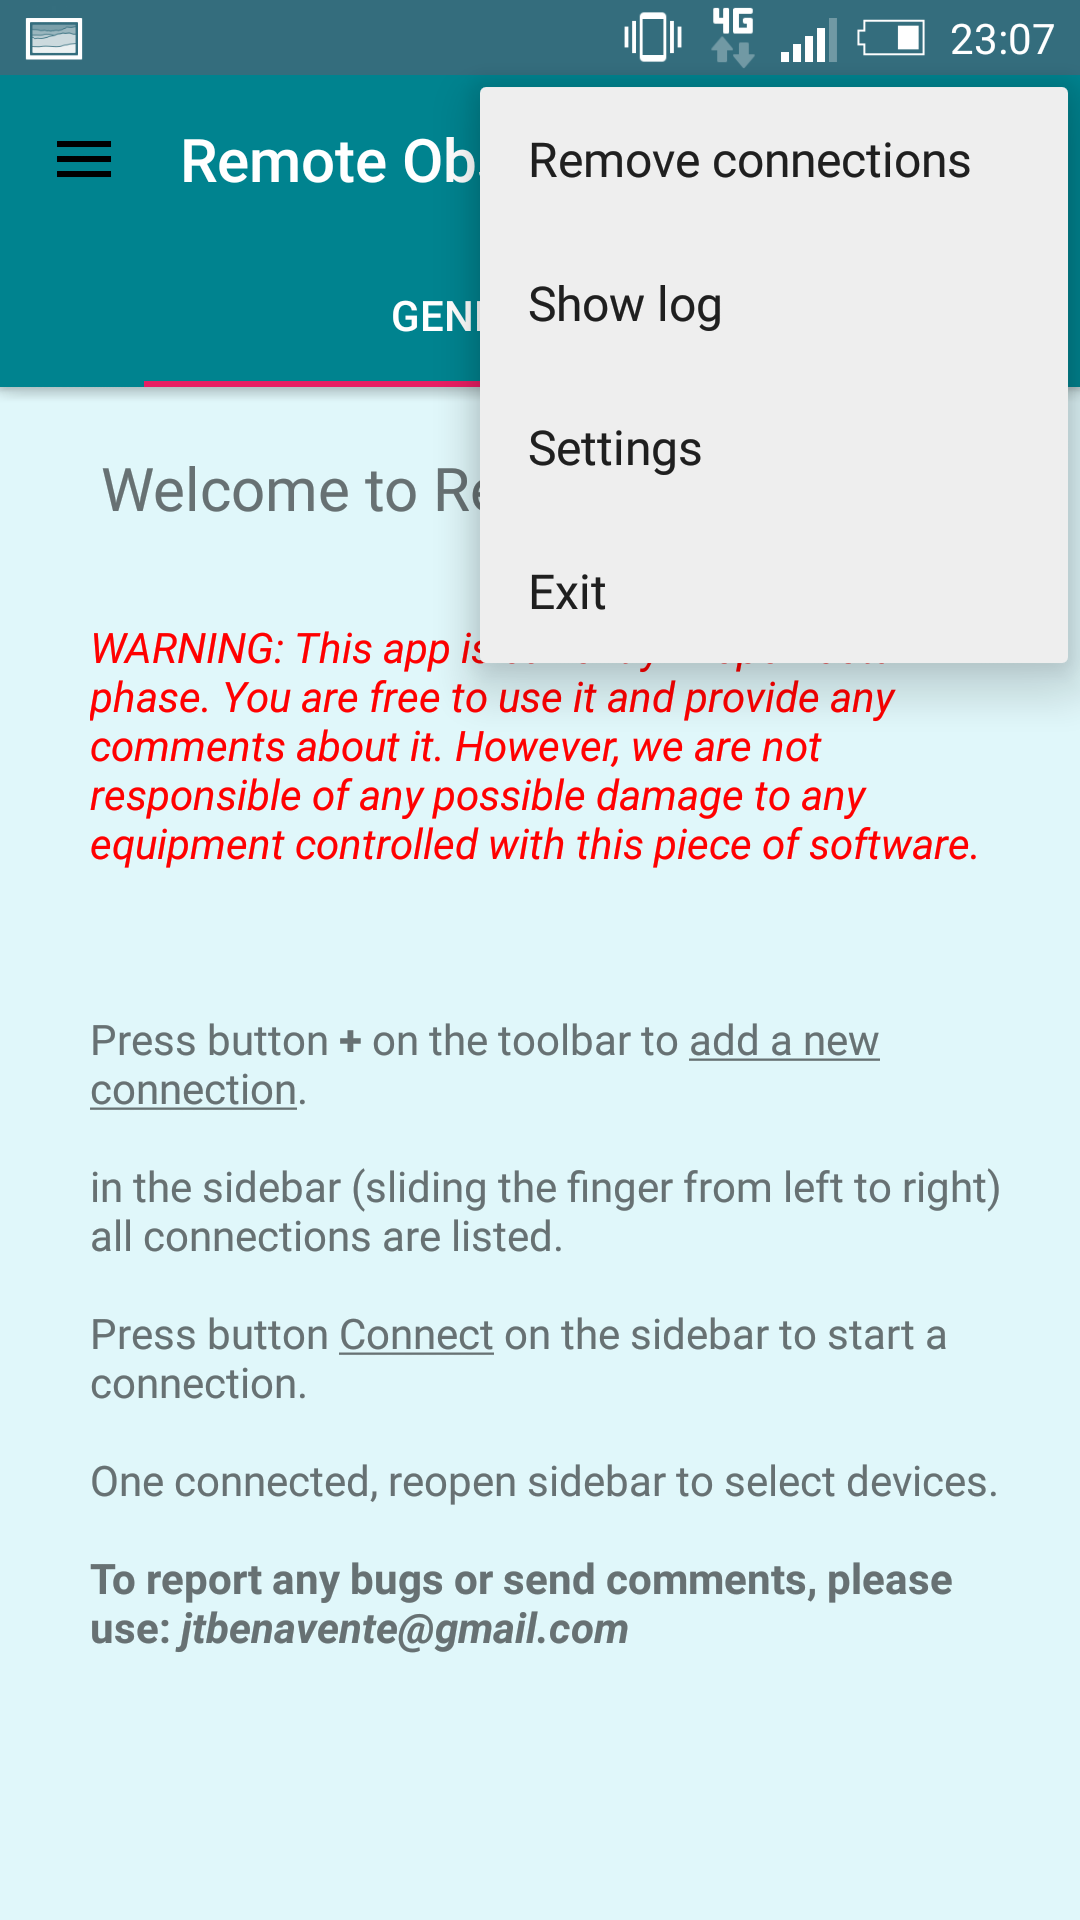
\includegraphics[width=\textwidth]{../images/captura8.png}
        \caption{}
        \label{fig:captura6}
    \end{subfigure}
    \begin{subfigure}[]{0.4\textwidth}
        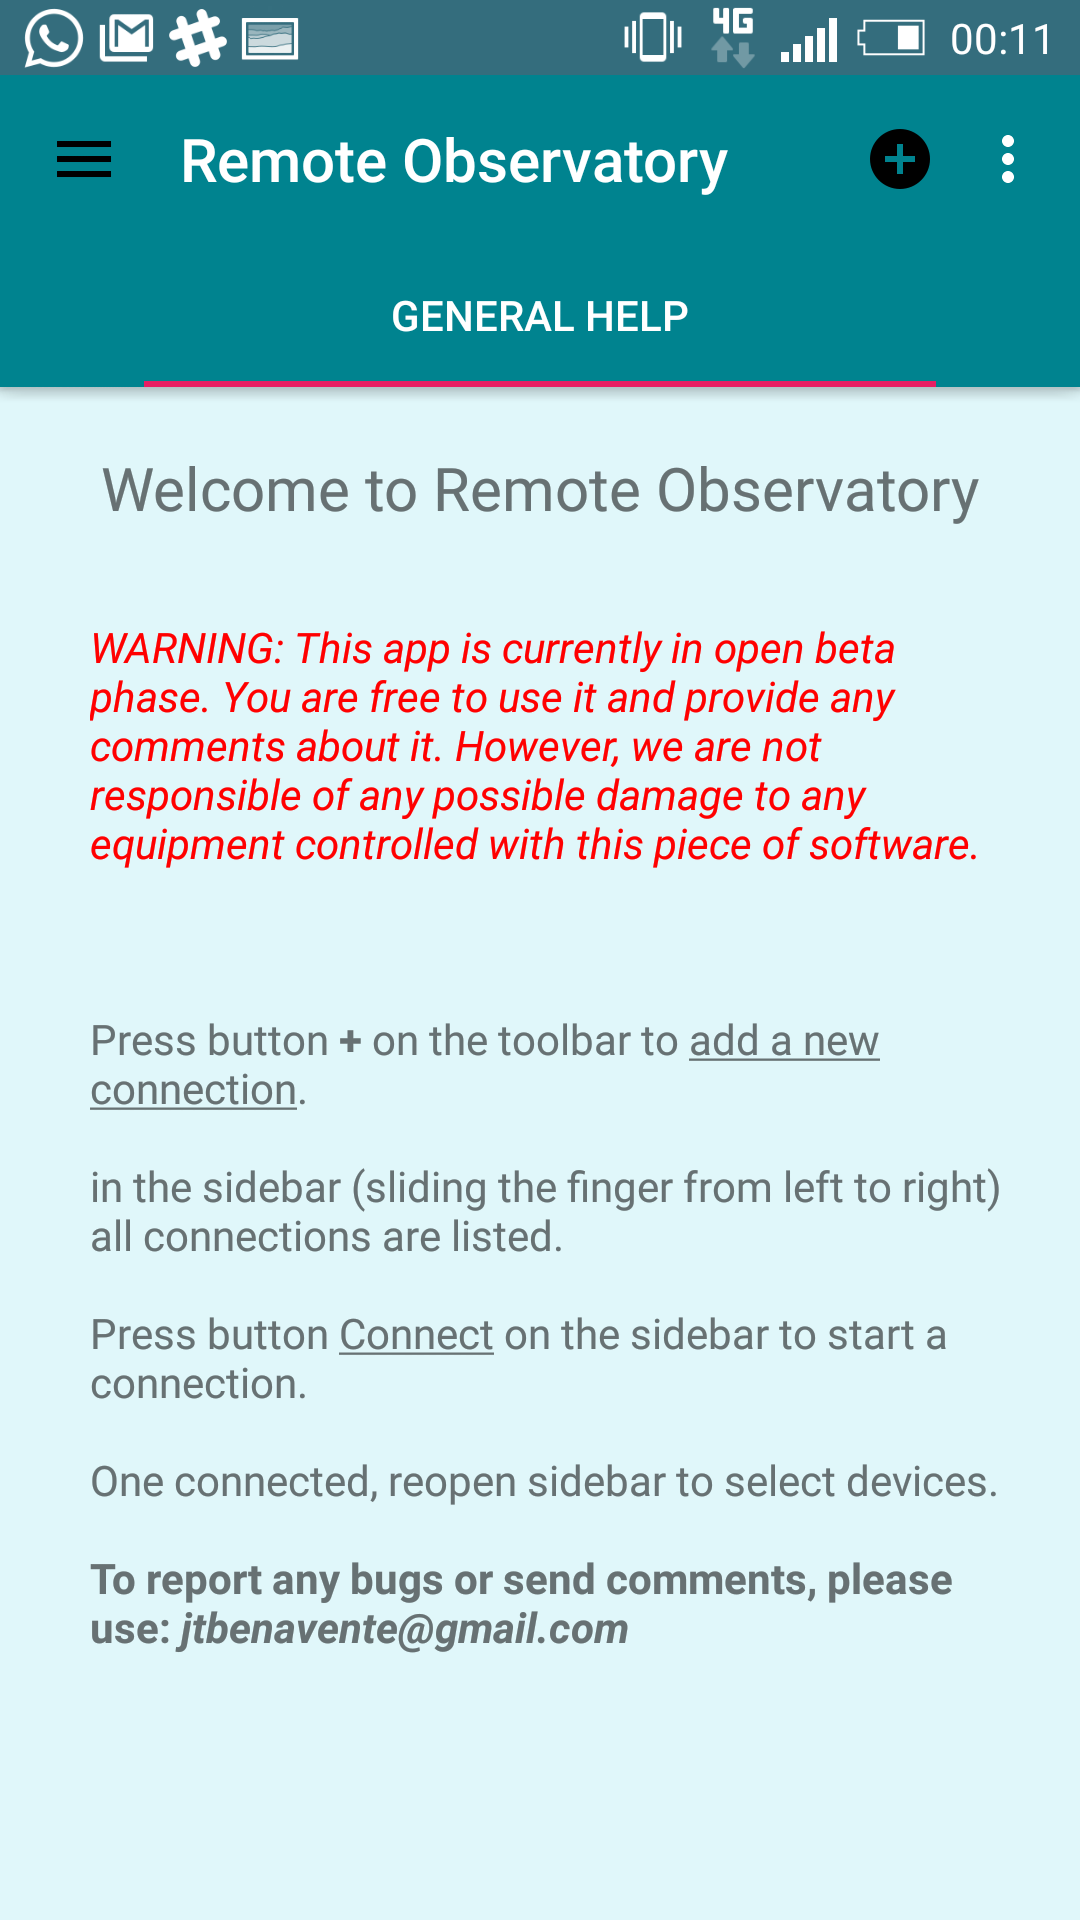
\includegraphics[width=\textwidth]{../images/captura9.png}
        \caption{}
        \label{fig:captura7}
    \end{subfigure}
    \caption{Capturas de la interfaz principal}\label{fig:capturas4}
\end{figure}


\bigskip
\subsection{Interfaz para listar las propiedades}

Una vez definido el aspecto general de la aplicación y los modos de navegación, el principal objetivo es poder listar las propiedades de los dispositivos. Desde las primeras reunión tuvimos claro que debíamos usar una lista estándar de \textbf{Android}, aunque debíamos abordar un tema importante: la posibilidad de agrupar las propiedades de un mismo grupo.
Hasta la \textbf{cuarta iteración} no se decidió utilizar la que a la postre sería la solución definitiva, \textbf{las listas expandibles}.

\begin{figure}
    \centering
    \begin{subfigure}[]{0.4\textwidth}
        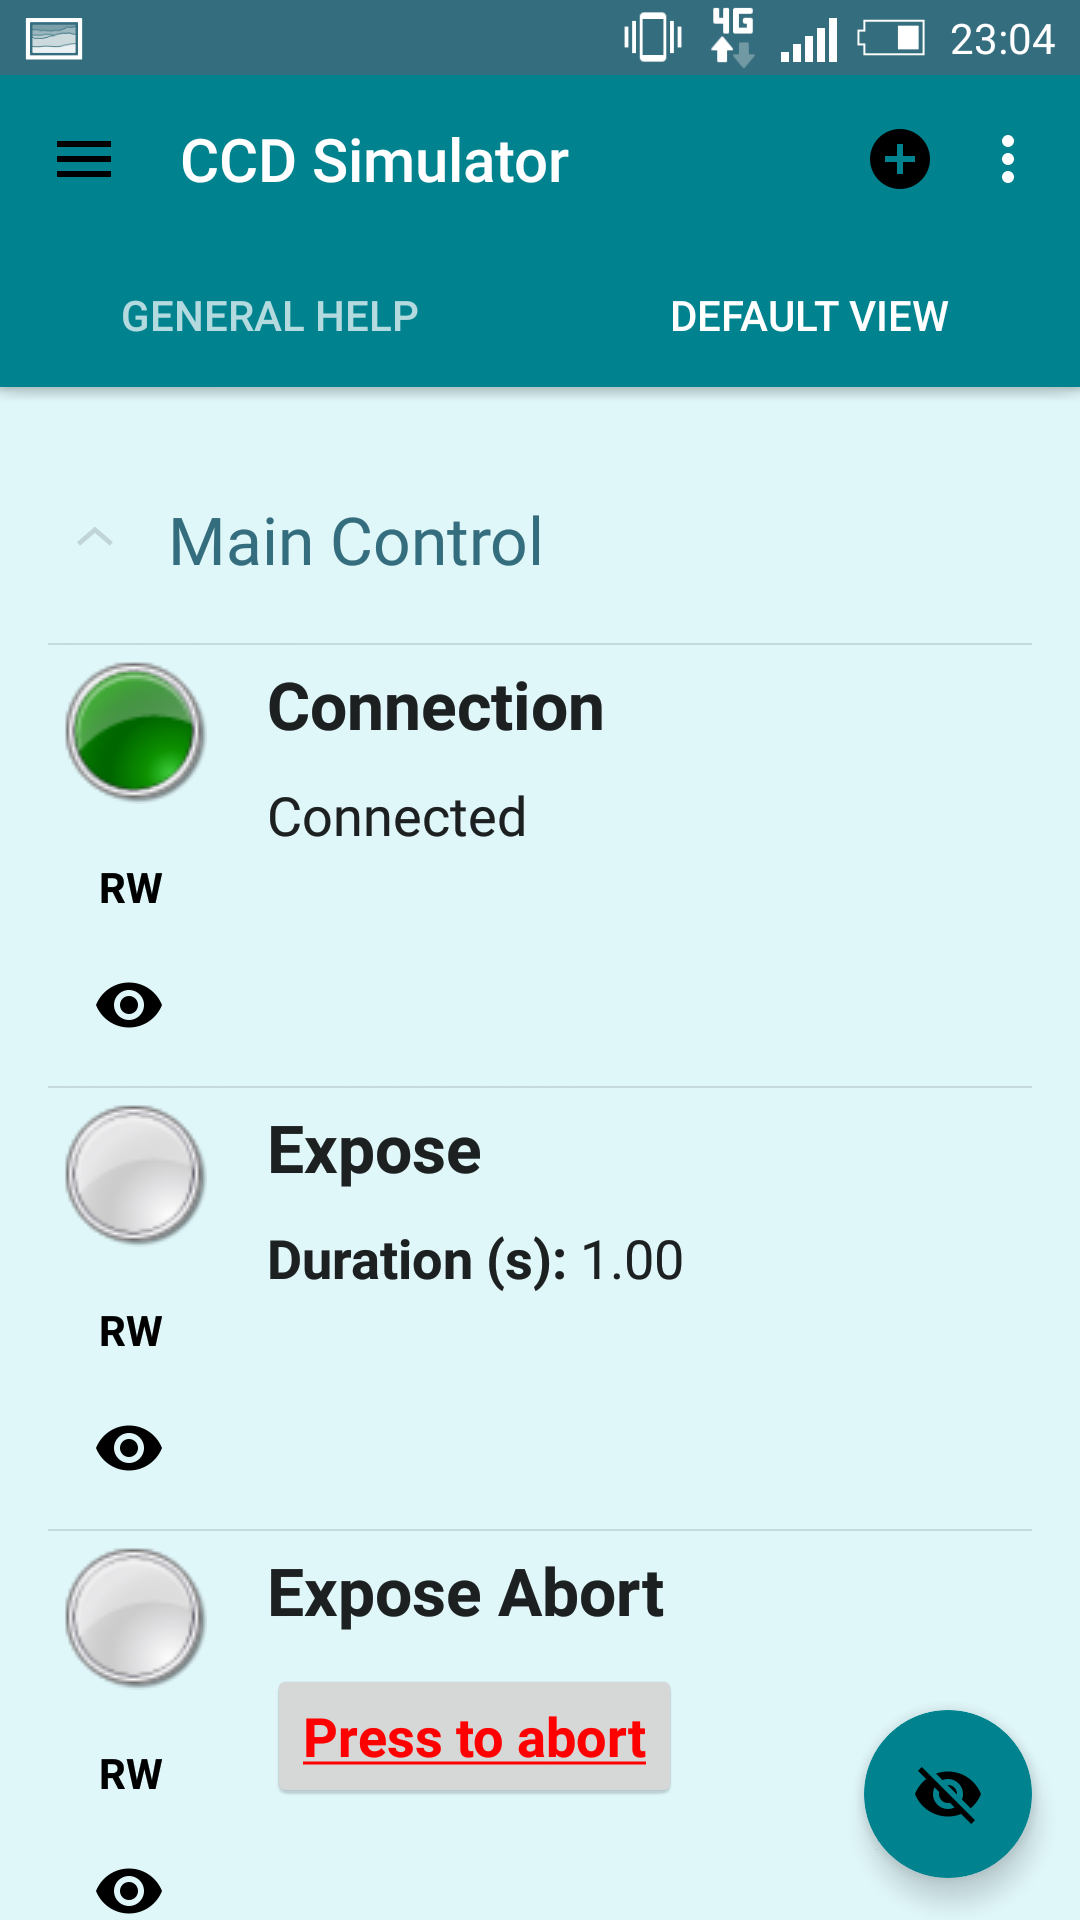
\includegraphics[width=\textwidth]{../images/captura10.png}
        \caption{}
        \label{fig:captura8}
    \end{subfigure}
    \begin{subfigure}[]{0.4\textwidth}
        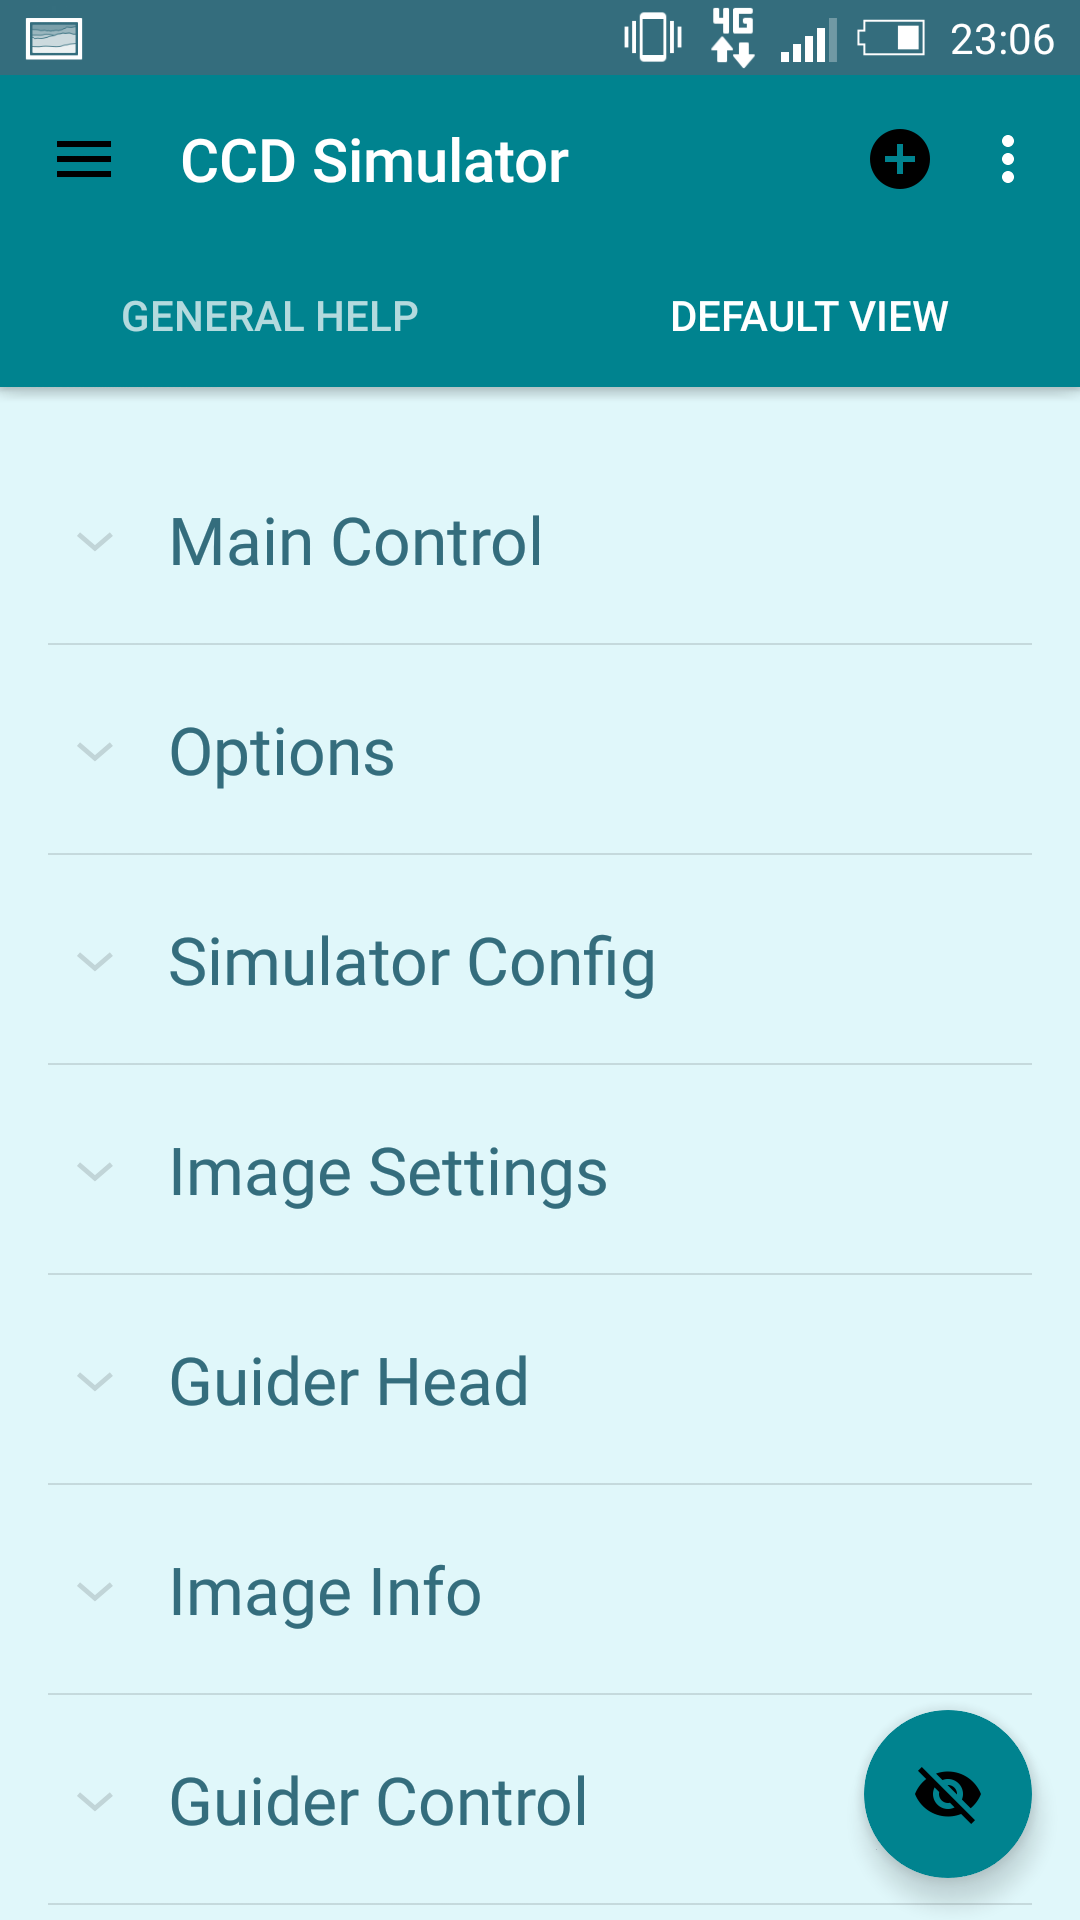
\includegraphics[width=\textwidth]{../images/captura11.png}
        \caption{}
        \label{fig:captura9}
    \end{subfigure}
    \caption{Lista de propiedades de un dispositivo}\label{fig:capturas5}
\end{figure}

En la figura \ref{fig:capturas5} podemos ver las listas con los grupos contraídos y extendidos. Además podemos ver como, en un nuevo esfuerzo por seguir las tendencias más actuales, se ha añadido un \textbf{botón flotante}\cite{ATMFAB} para mostrar u ocultar las propiedades con visibilidad ``oculta''.


\bigskip
\subsection{Interfaz de propiedad}
Una vez definida la lista de las propiedades, abordamos el problema de la interfaz para una propiedad. Para ello analizamos todos los elementos en común y todas las diferencias entre los distintos tipos de propiedades. En la figura \ref{fig:captura4} podemos ver la parte común a todas las propiedades:

\begin{itemize}
  \item \textbf{Nombre de la propiedad.}
  \item \textbf{Estado de la propiedad.}
  \item \textbf{Permisos de escritura y/o lectura.}
  \item \textbf{Visibilidad.}
\end{itemize}

Todas las propiedades comparten estos cuatro elementos, siendo la parte central de la vista la que se adaptará según el tipo.

\bigskip
\subsubsection{Text, Number y Switch}

De cara a los items de la lista, las propiedades \textit{text y number} son idénticas salvo que el valor de los elementos del primero son texto y del segundo son números. Cada elemento se coloca debajo del anterior creando otra lista (una propiedad puede tener uno o más elementos).

En la figura \ref{fig:capturas6} podemos ver ambas vistas en la interfaz de las propiedades. 


\begin{figure}
    \centering
    \begin{subfigure}[]{0.4\textwidth}
        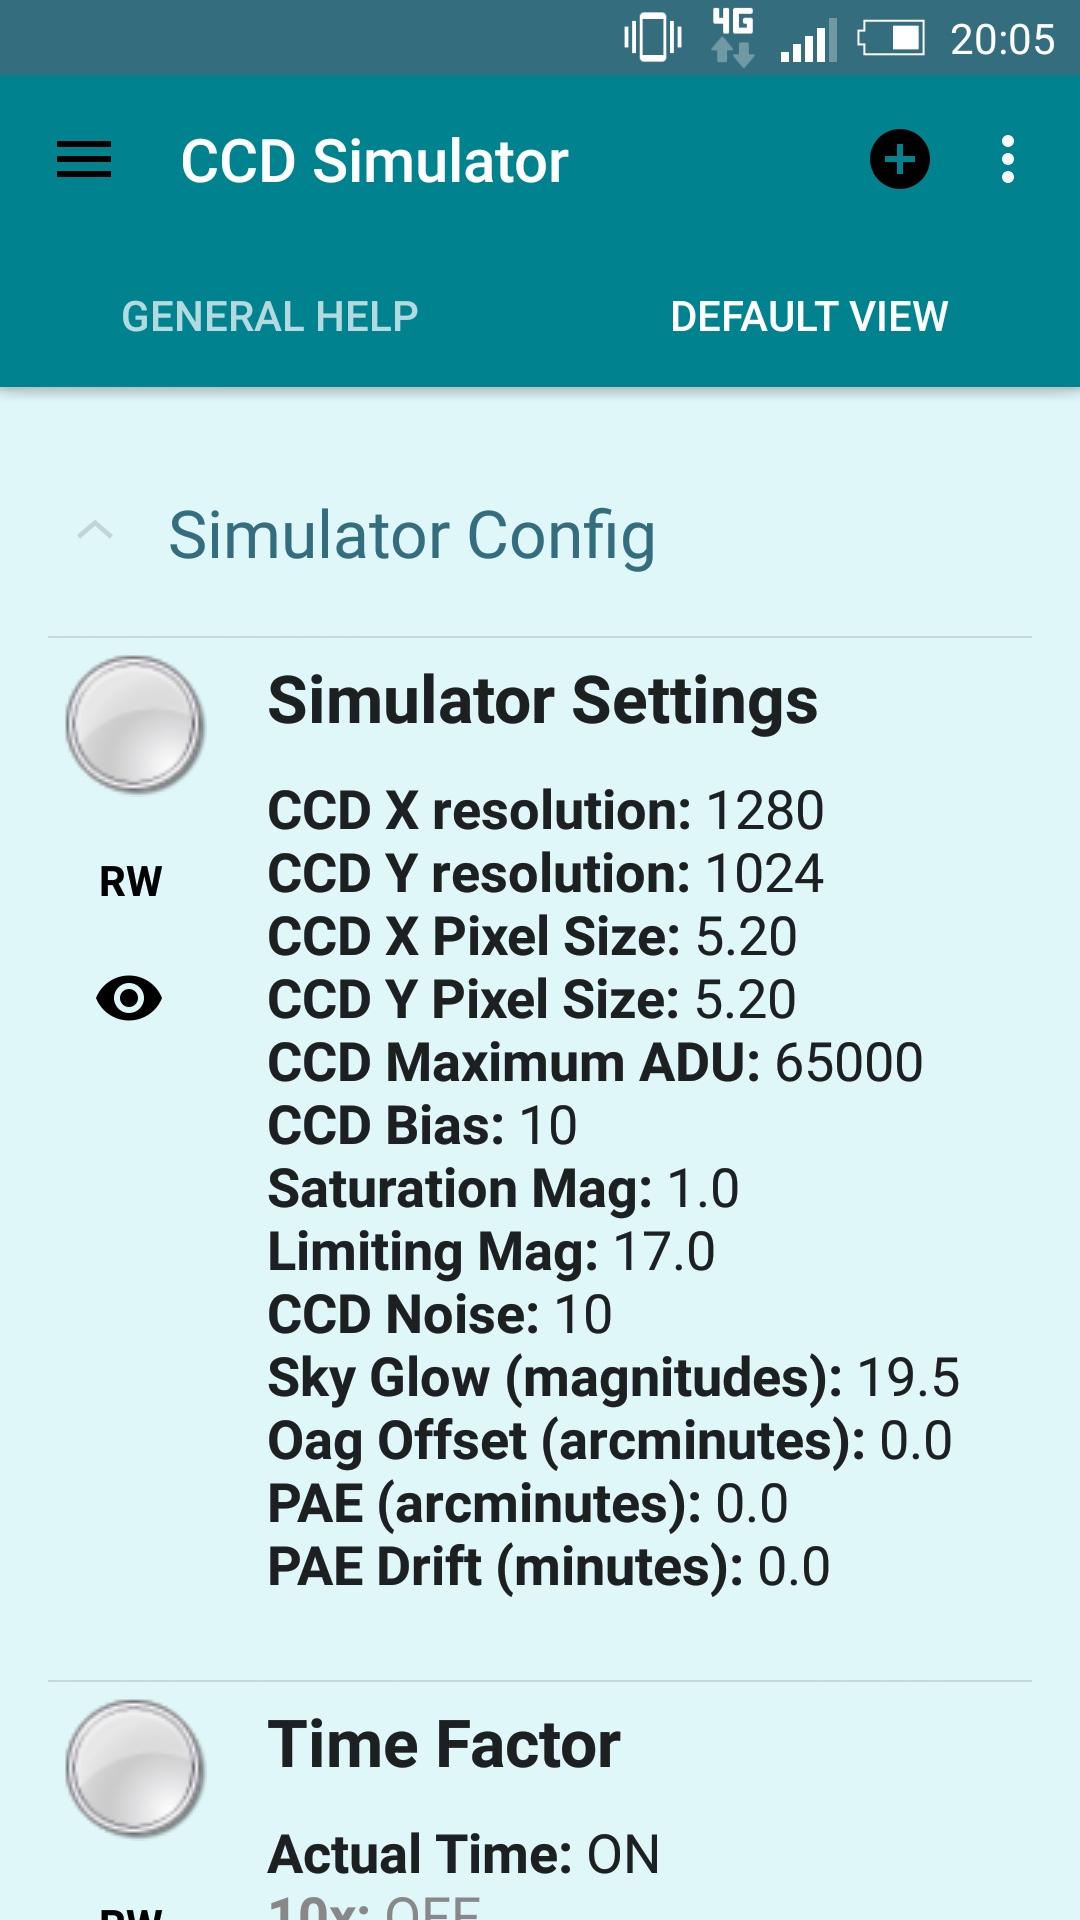
\includegraphics[width=\textwidth]{../images/captura12.png}
        \caption{}
        \label{fig:captura10}
    \end{subfigure}
    \begin{subfigure}[]{0.4\textwidth}
        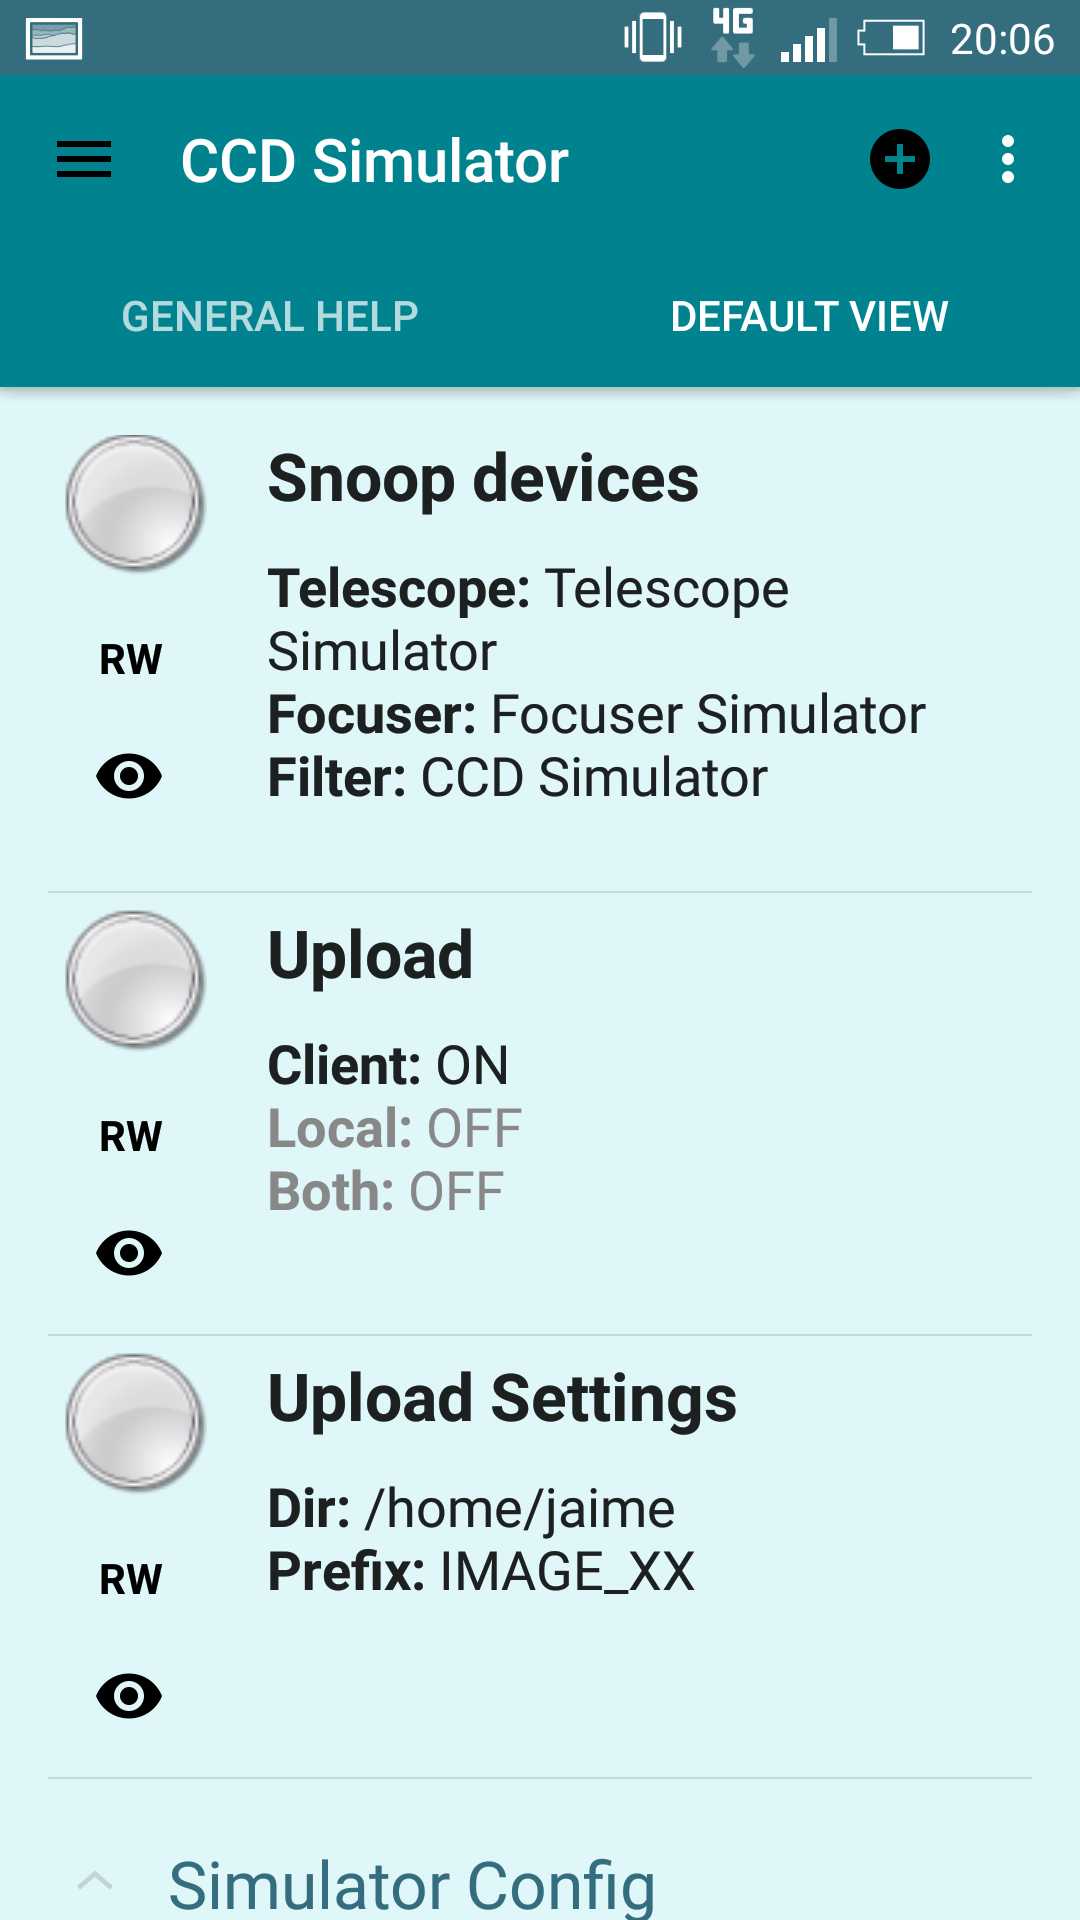
\includegraphics[width=\textwidth]{../images/captura13.png}
        \caption{}
        \label{fig:captura11}
    \end{subfigure}
    \caption{Propiedades text, number y switch}\label{fig:capturas6}
\end{figure}

Los \textit{Switch} tienen una vista similar a las dos propiedades anteriores, salvo que el valor que está en estado ``on'' en negro y los que están en estado ``off'' en gris (figura \ref{fig:capturas6}).


\bigskip
\subsubsection{Blobs}
Los \textit{Switch} son ficheros enviados por el servidor por lo que es más interesante mostrar el tipo de archivo que recibimos y su tamaño. Como se puede ver en la figura \ref{fig:blob}, además de estos dos datos tenemos los botones para poder guardarlo o enviarlo a \textbf{Android} para poder abrirlo con la aplicación adecuada.

\bigskip
\begin{figure}[!ht]
  \begin{center}
  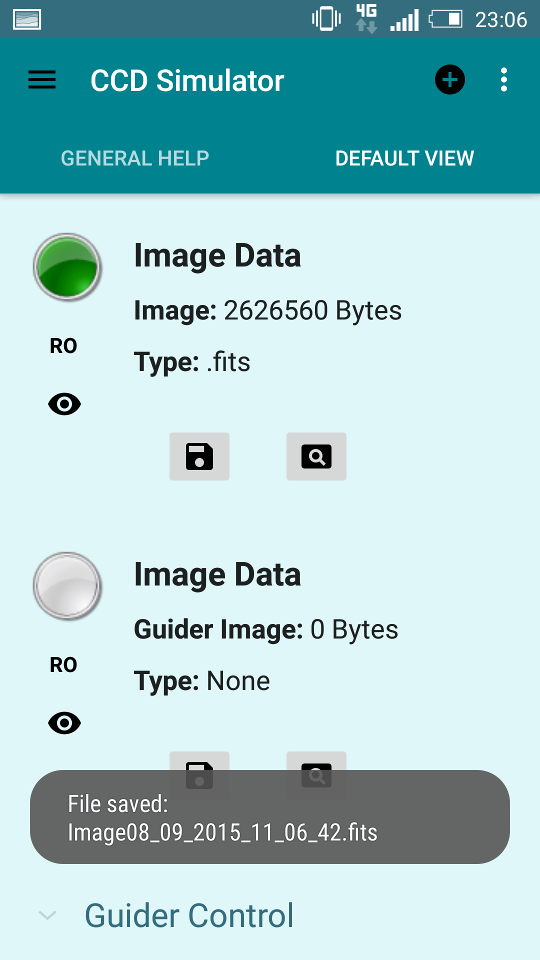
\includegraphics[width=0.3\textwidth]{../images/saveBlob2.png}
  \caption{Vista de un Blob}
  \label{fig:blob}
  \end{center}
\end{figure}

\bigskip
\subsubsection{Light}
Esta propiedad es muy similar a los \textit{switch} salvo que el valor de cada uno de los elementos de la propiedad será un icono representando una luz roja, verde, gris o amarilla.


\bigskip
\subsection{Interfaz de diálogos}

Los diálogos son una herramienta visual esencial que permiten superponer una vista para llamar la atención del usuario, bien sea para informar o para ejecutar alguna acción como editar propiedades.


\bigskip
\subsubsection{Diálagas para editar propiedades}

Estos diálogos permiten editar los elementos de aquellas propiedades que lo permitan:

\begin{itemize}
  \item \textbf{Dialogo de edición de una propiedad Text:} Se muestra la lista de elementos con su \textit{label} y su valor en un cuadro editable (\ref{fig:text_edit}).
  \item \textbf{Dialogo de edición de una propiedad Number:} Se muestra la lista de elementos con su \textit{label} y sus valores máximos y mínimos. Debajo se puede ver el campo editable con el valor (\ref{fig:number_edit}).
  \item \textbf{Dialogo de edición de una propiedad Switch:} Se muestra cada elemento con su \textit{label} seguido de un botón de estados para indicar si el elemento está activo (``on'') o no (``off'') (\ref{fig:number_edit}) .
\end{itemize}


\begin{figure}[!ht]
  \begin{center}
  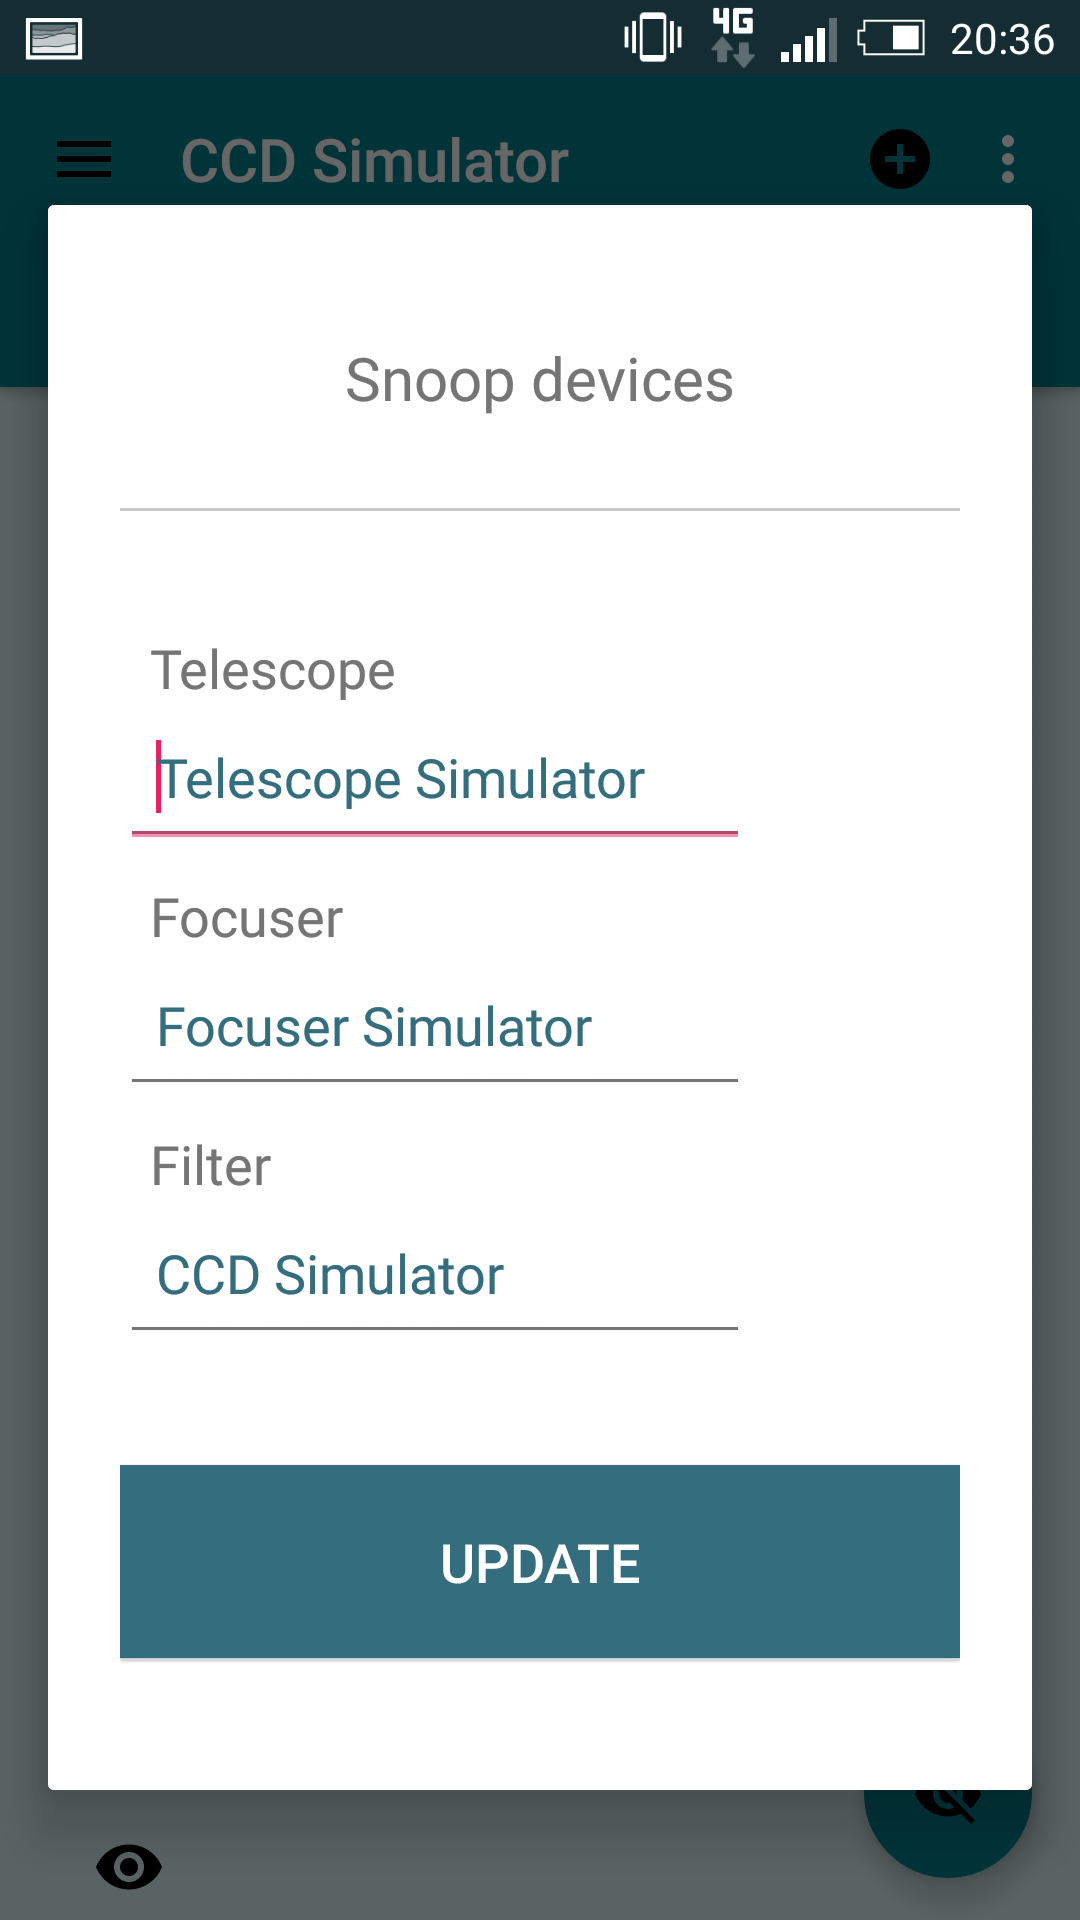
\includegraphics[width=0.3\textwidth]{../images/text_edit_view.png}
  \caption{Dialogo para editar una propiedad text}
  \label{fig:text_edit}
  \end{center}
\end{figure}


\begin{figure}[!ht]
  \begin{center}
  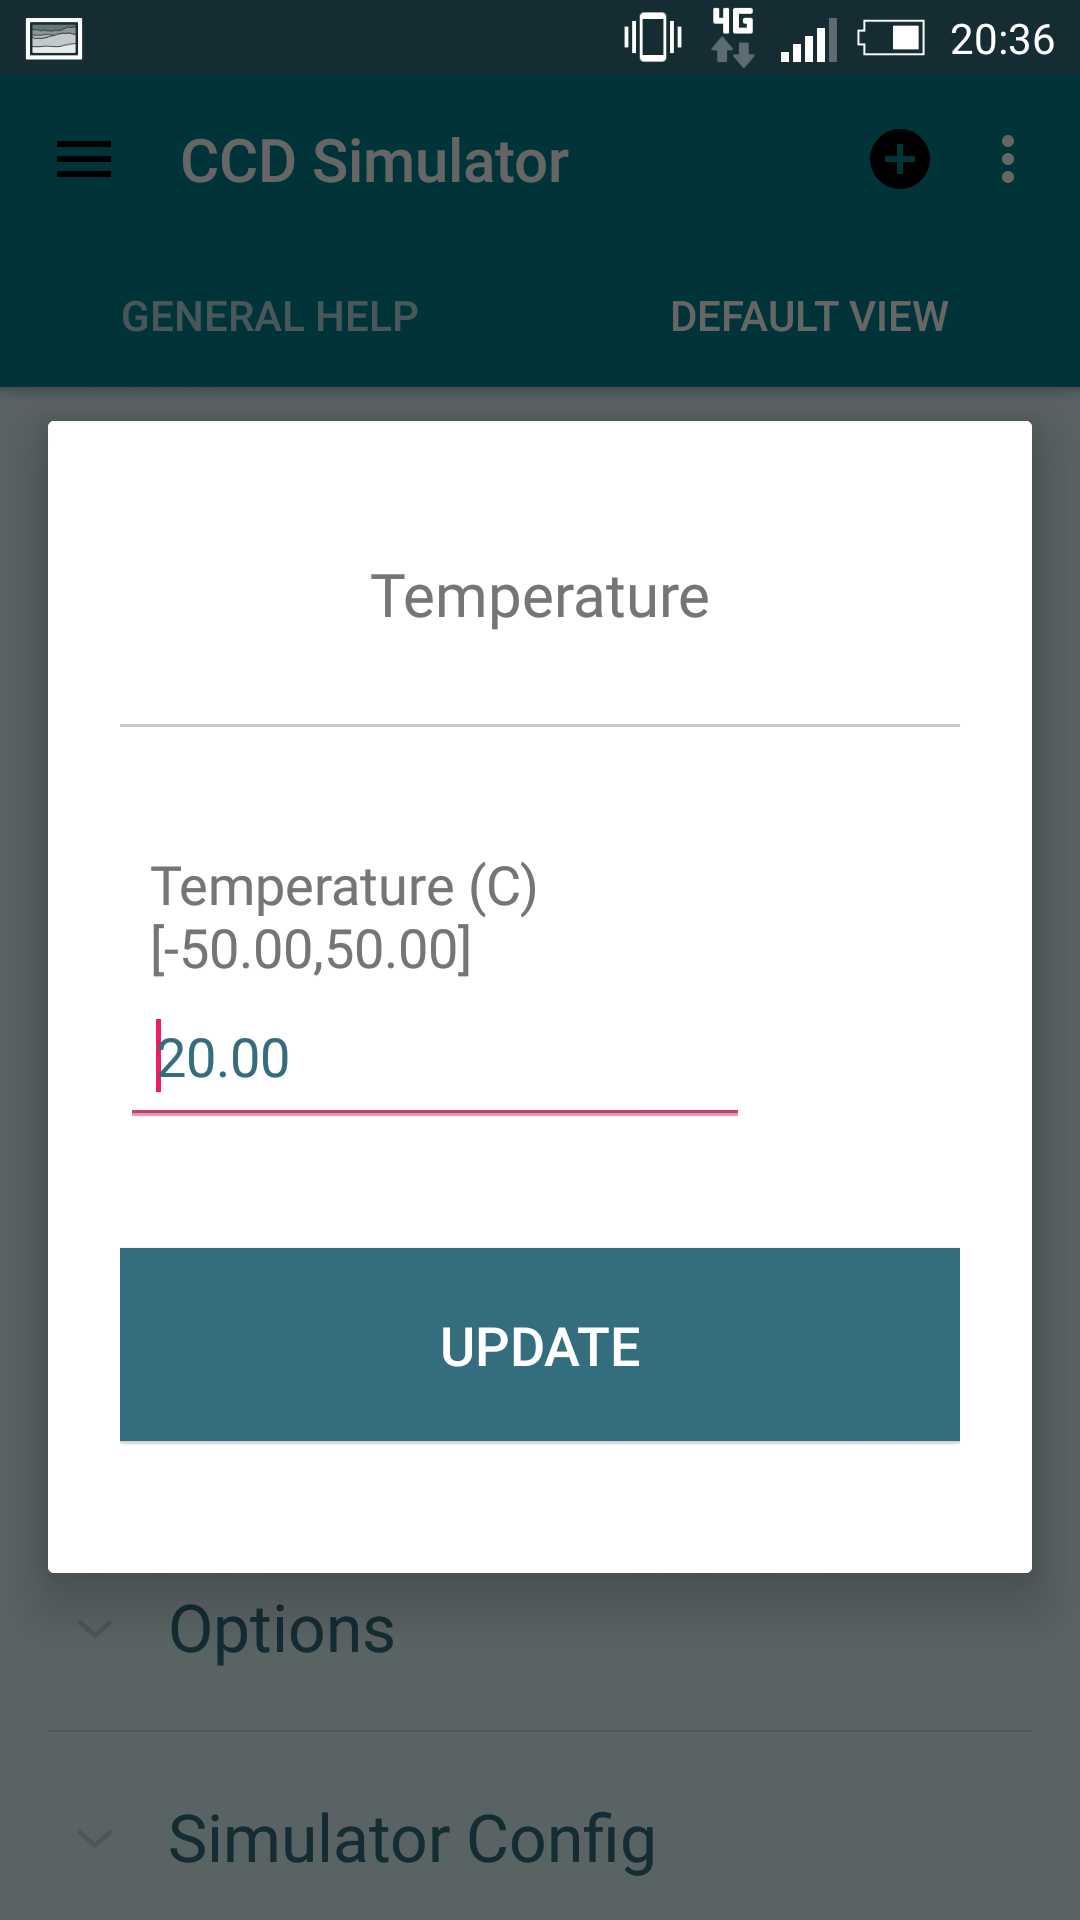
\includegraphics[width=0.3\textwidth]{../images/number_edit_view.png}
  \caption{Dialogo para editar una propiedad number}
  \label{fig:number_edit}
  \end{center}
\end{figure}


\begin{figure}[!ht]
  \begin{center}
  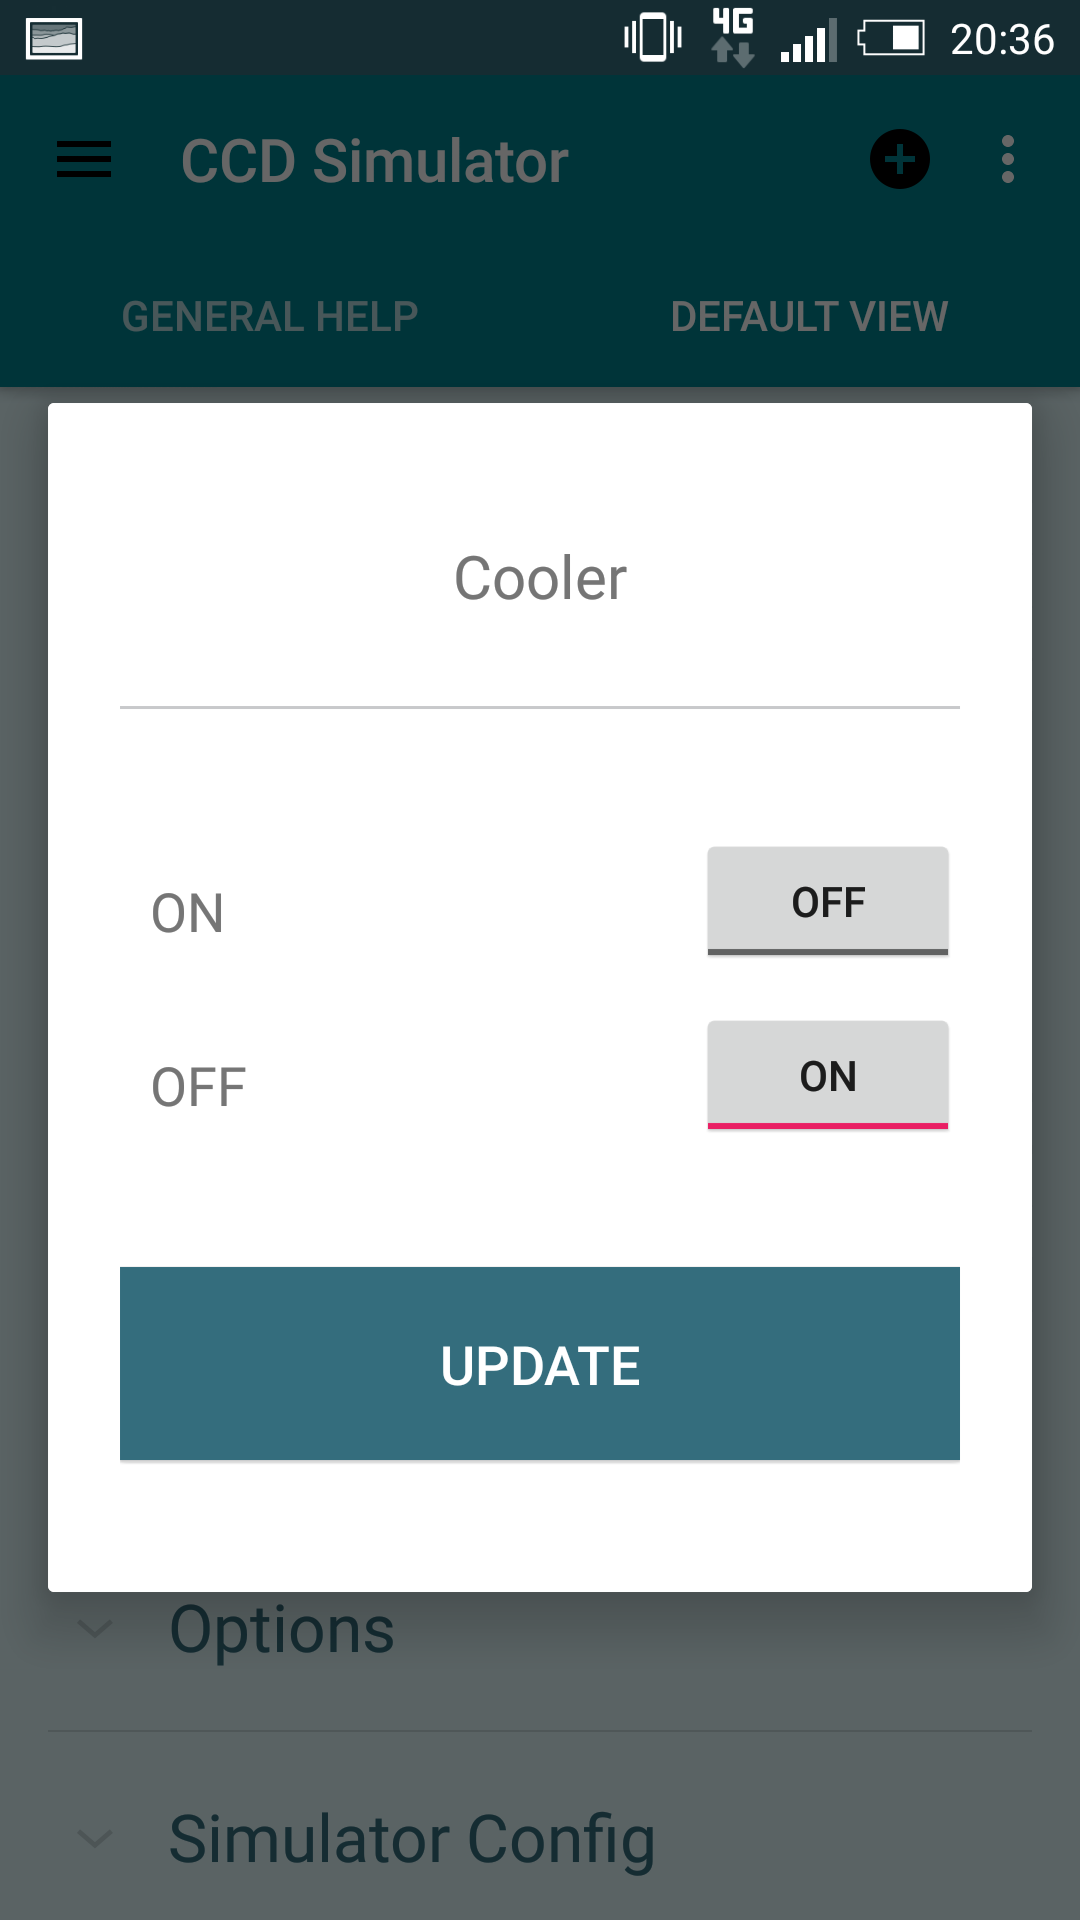
\includegraphics[width=0.3\textwidth]{../images/switch_edit_view.png}
  \caption{Dialogo para editar una propiedad switch}
  \label{fig:number_edit}
  \end{center}
\end{figure}

\bigskip
\subsubsection{Diálogos para gestión de las conexiones}

Estos diálogos permiten añadir, editar o borrar conexiones. Como cada conexión se define por un nombre, un URL del servidor, un puerto y las opciones de activar la recepción de blobs y la autoconexión, todos estos campos son comunes a la vista para añadir y para editar. La vista para editar añade un botón para poder borrar el log de la conexión (figuras \ref{fig:new_connect} y \ref{fig:edit_connect}).


\begin{figure}[!ht]
  \begin{center}
  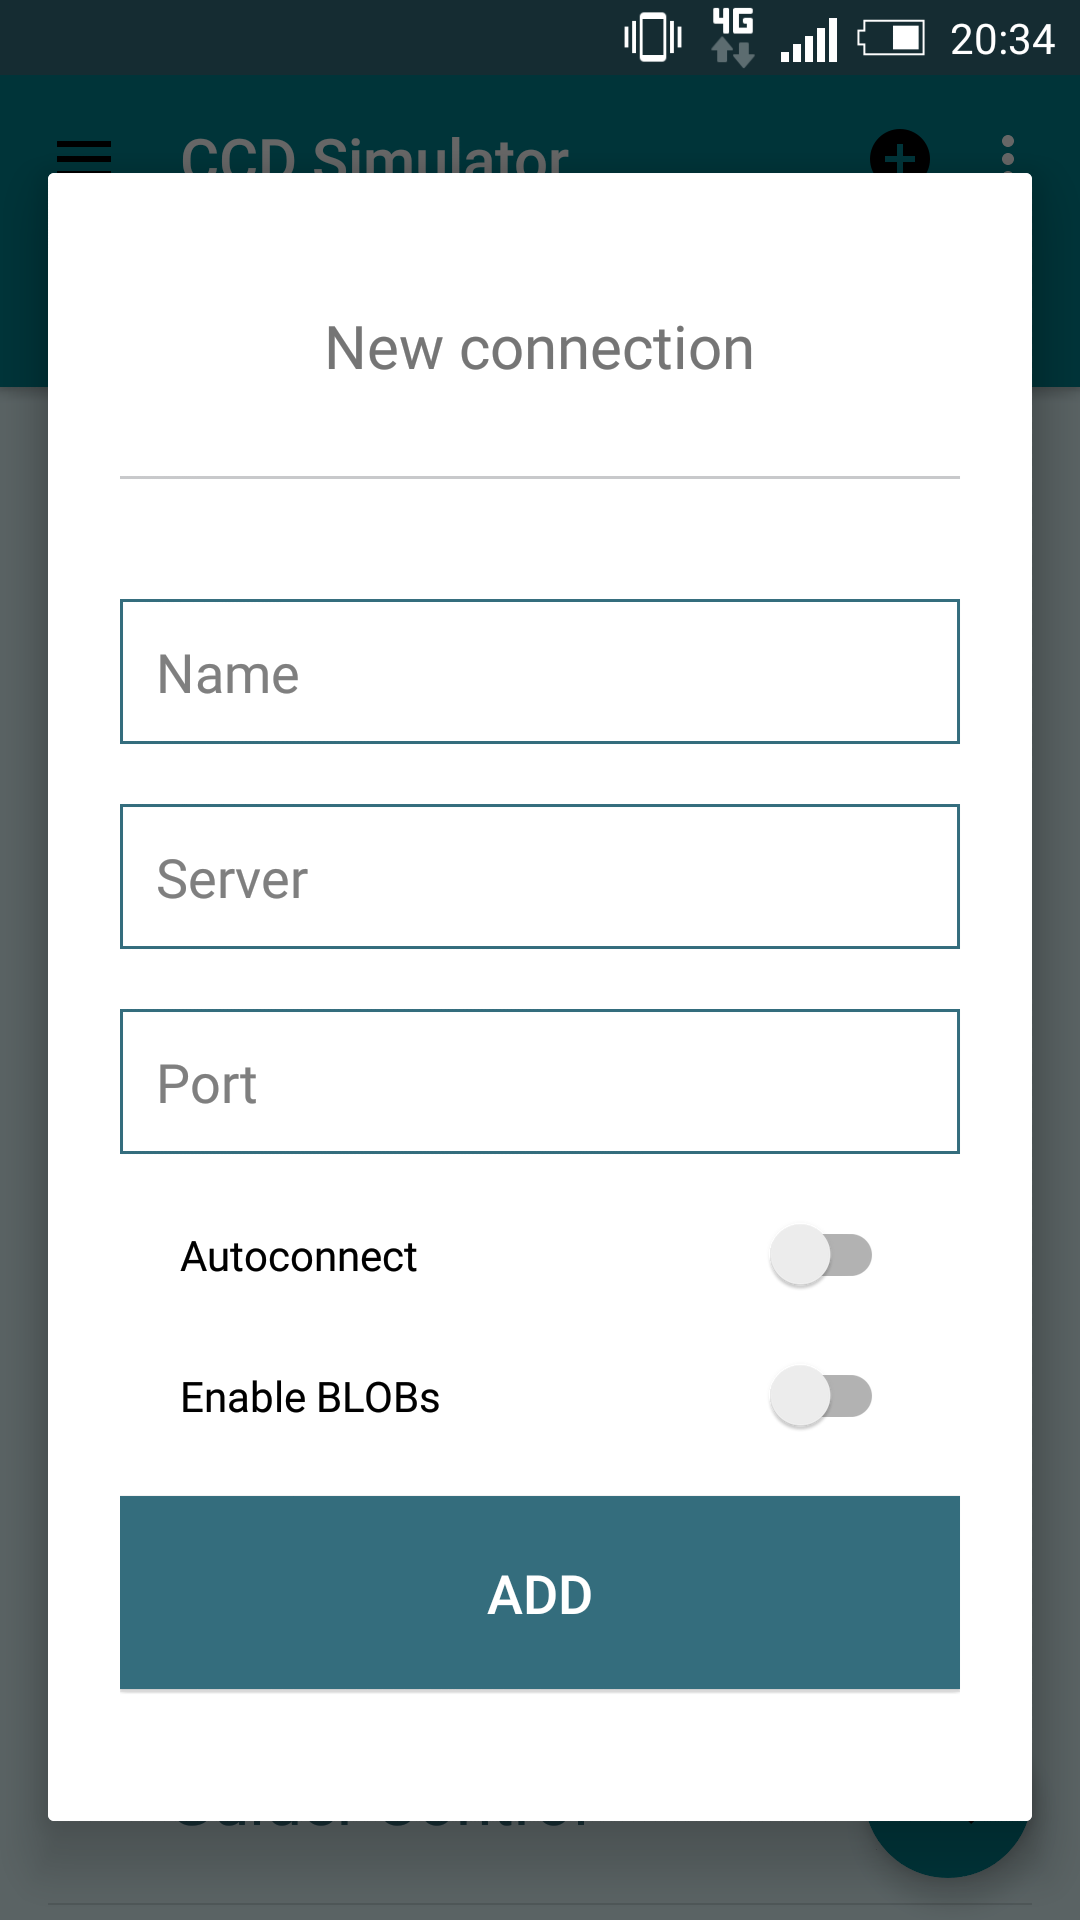
\includegraphics[width=0.3\textwidth]{../images/nueva_conexion.png}
  \caption{Dialogo para añadir una conexión}
  \label{fig:new_connect}
  \end{center}
\end{figure}


\begin{figure}[!ht]
  \begin{center}
  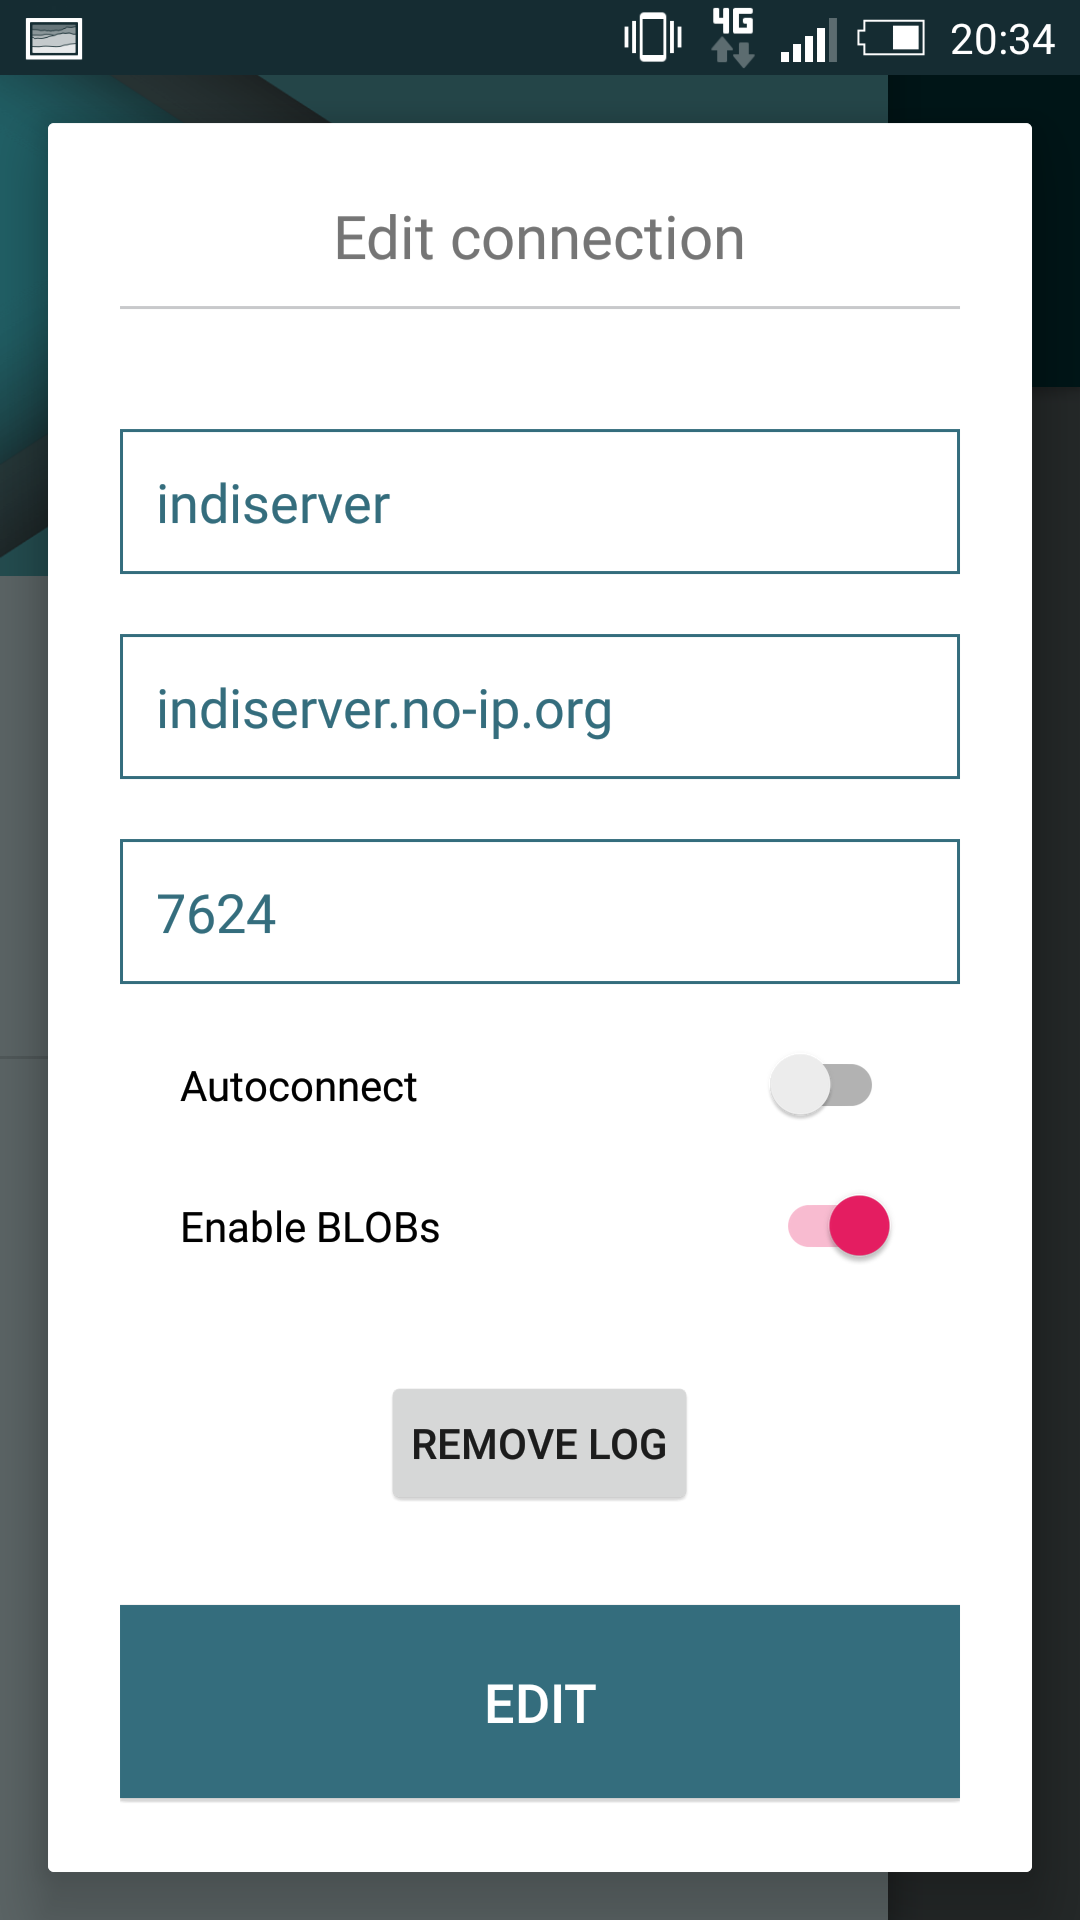
\includegraphics[width=0.3\textwidth]{../images/editar_conexion.png}
  \caption{Dialogo para editar una conexión}
  \label{fig:edit_connect}
  \end{center}
\end{figure}

\bigskip
La vista para borrar conexiones es una simple lista con todas las conexiones que haya y un \textit{checkbox} para marcar las que deseamos borrar (figura \ref{fig:remove_connect}).


\begin{figure}[!ht]
  \begin{center}
  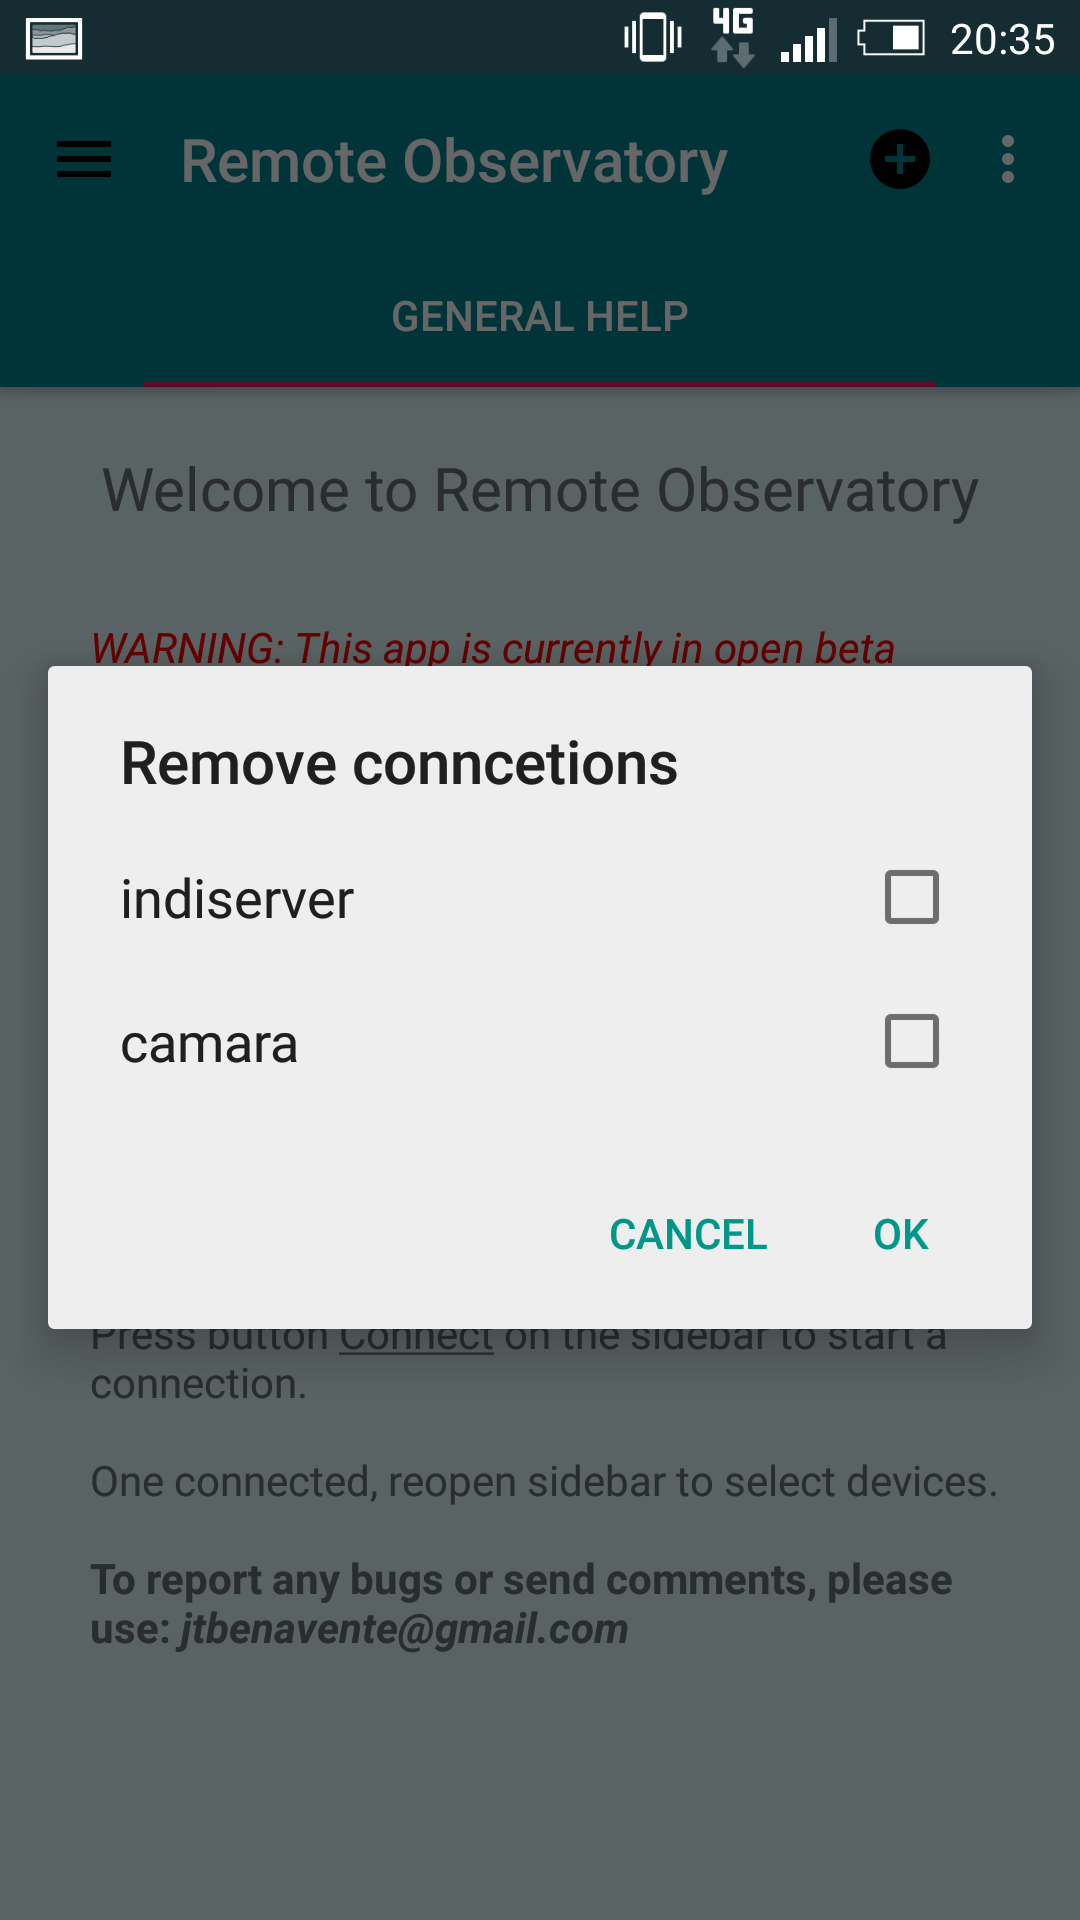
\includegraphics[width=0.3\textwidth]{../images/borrar_conexiones.png}
  \caption{Dialogo para borrar conexiones}
  \label{fig:remove_connect}
  \end{center}
\end{figure}


\bigskip
\subsubsection{Diálogos para informar de errores o avisos}
Estas vistas informan al usuario de un error al introducir datos, errores de desconexión o conexión y de alerta cuando se añaden o quitan nuevos dispositivos (\ref{fig:alert_view}).

\begin{figure}[!ht]
  \begin{center}
  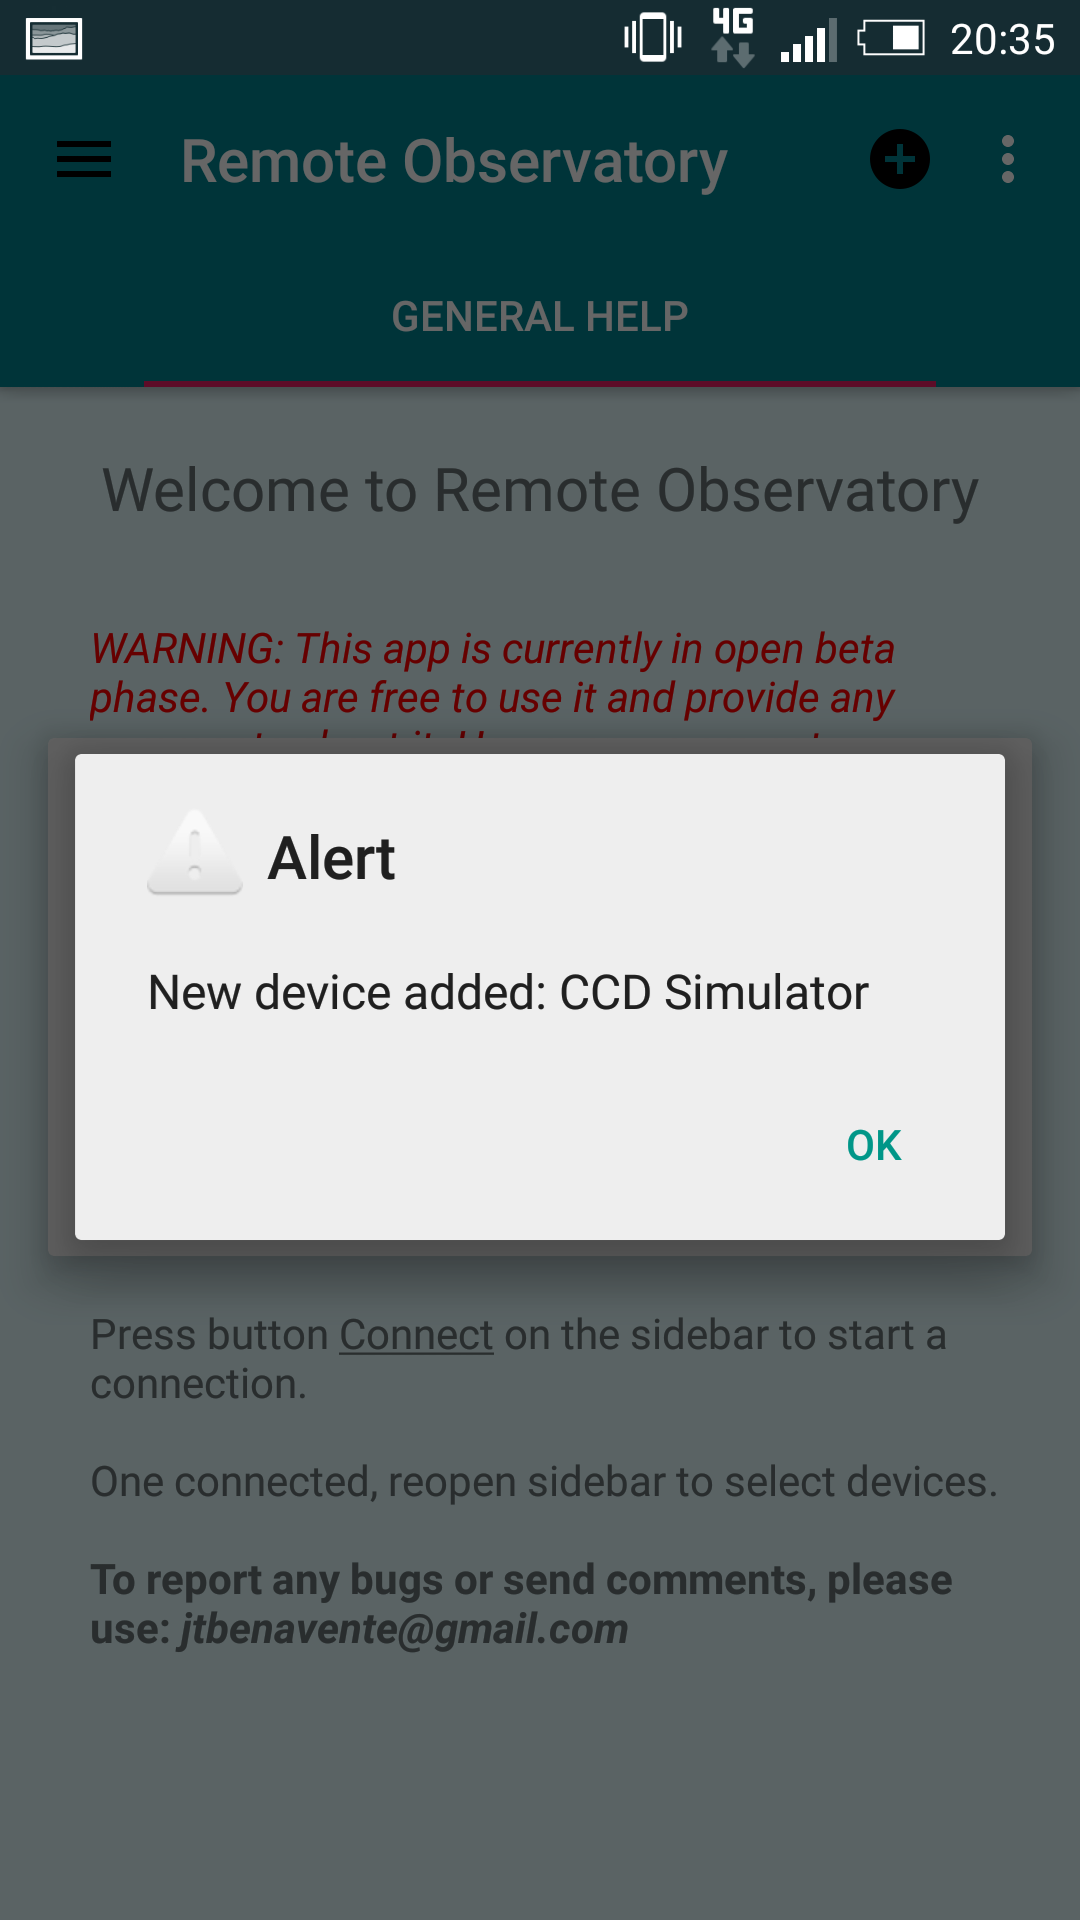
\includegraphics[width=0.3\textwidth]{../images/aviso.png}
  \caption{Dialogo de aviso}
  \label{fig:alert_view}
  \end{center}
\end{figure}


\bigskip
\subsection{Interfaz de log}

Esta es una interfaz muy simple para poder ver los \textit{logs} de cada una de las conexiones guardadas en la aplicación. Para ello se crea una vista tabulada con todas ellas (figura \ref{fig:log_view}).

\begin{figure}[!ht]
  \begin{center}
  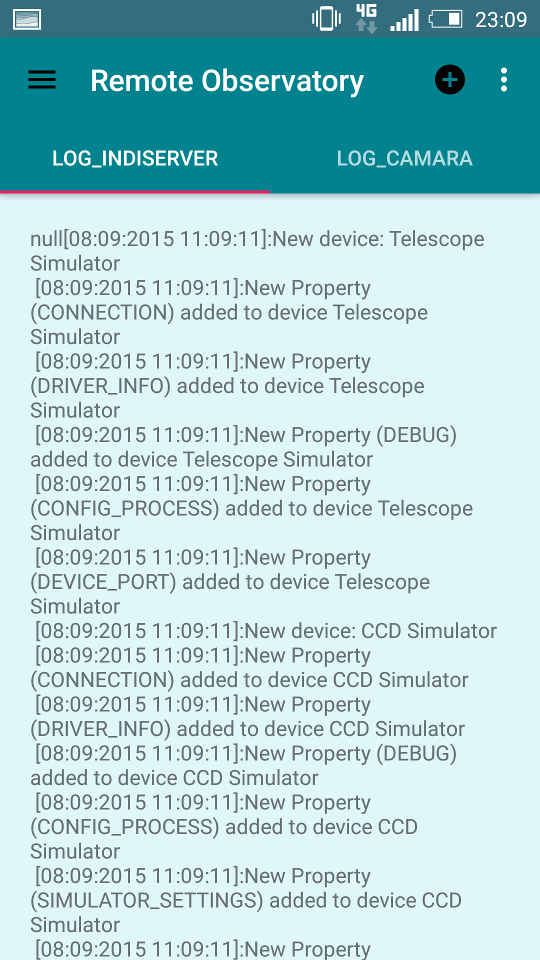
\includegraphics[width=0.3\textwidth]{../images/log2.png}
  \caption{Vista de los ajustes}
  \label{fig:log_view}
  \end{center}
\end{figure}


\bigskip
\subsection{Interfaz de los ajustes}

Los ajustes tienen una vista especial para poder editar las diferentes notificaciones y para poder establecer una carpeta para almacenar los archivos de la aplicación. Como podemos ver en la figura \ref{fig:settings_view}, cada una de las notificaciones tienen un elemento \textit{switch} de \textbf{Android} para marcar el estado. Al final de la vista encontramos un campo editable para poner la ruta que deseemos para la carpeta.


\begin{figure}[!ht]
  \begin{center}
  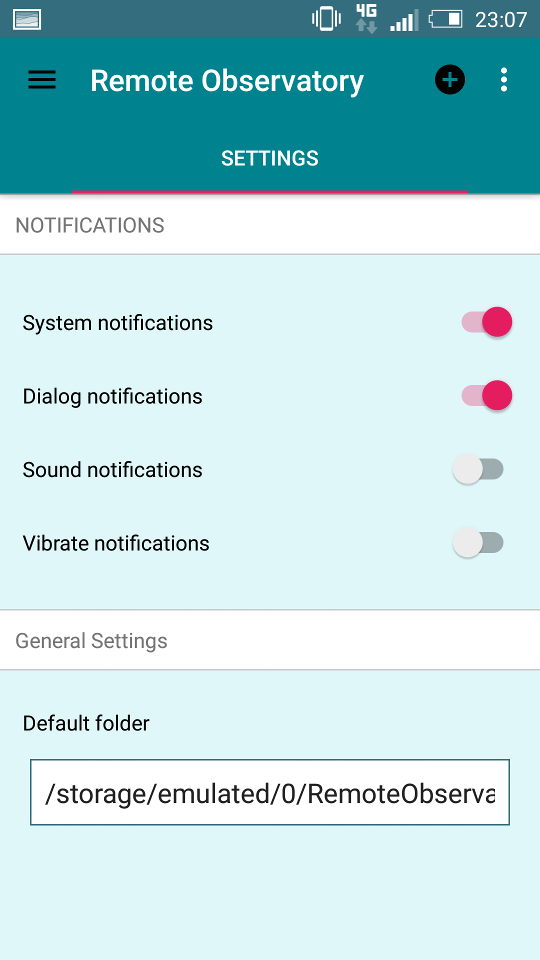
\includegraphics[width=0.3\textwidth]{../images/settings2.png}
  \caption{Vista de los ajustes}
  \label{fig:settings_view}
  \end{center}
\end{figure}


\bigskip
\section{Mecanismo de adición de vistas}

Uno de los objetivos principales del proyecto es facilitar a desarrolladores externos al proyecto, la posibilidad de agregar nuevas clases para gestionar vistas especificas de propiedades y dispositivos, liberando al desarrollador de la necesidad de conocer el código de la aplicación. Para ello se han diseñado una serie de mecanismos y pasos a seguir para poder añadir vistas personalizadas.


\bigskip
\subsection{Propiedades}
Para poder añadir una nueva vista debemos seguir tres pasos:

\begin{itemize}
  \item Crear una clase que implemente la interfaz \textbf{UIPropertyManager}.
  \item Crear una interfaz de usuario para android en XML tanto para la vista de elemento de lista como para la vista para editar una propiedad.
  \item Declarar un objeto de la clase creada y añadirlo al vector de manejadores.
\end{itemize}


\subsubsection{Interfaz UIPropertyManager}

En la sección de diseño de clases hemos podido ver la interfaz que permite crear los distintos tipos de manejadores de propiedades.

\begin{lstlisting}[language=Java,caption={Interfaz UIPropertyManager},label={lst:ui_prop_manager}]

/**
 *  Interface to handle views and indi propertys
 */
public interface UIPropertyManager {
    /**
     *  Check if this class can represent p
     *
     * @param p Indi property
     * @return True/false if class can represent p
     */
    boolean handlesProperty (INDIProperty p);

    /**
     *  Create and return a view sets with p elements
     *
     * @param p Indi property
     * @param inflater Layout inflater to inflate view
     * @param parent ViewGroup to inflate view
     * @param context Context to allow use Activity methods
     * @return View
     */
    View getPropertyView (INDIProperty p, LayoutInflater inflater, ViewGroup parent, Context context);

    /**
     *  update view v with Indi property p elements
     *
     * @param p Indi property
     * @param v View
     */
    void updateView (INDIProperty p, View v);

    /**
     *  Create a new view dialog to allow set Indi property p elements
     *
     * @param p Indi property
     * @param inflater Layout inflater to inflate view
     * @return View
     */
    View getUpdateView(INDIProperty p, LayoutInflater inflater, DialogFragment fragment);

    /**
     *  Update property with change saved at view v
     *
     * @param p Indi property
     * @param v View
     */
    void updateProperty(INDIProperty p, View v);

    /**
     *  Get priority
     *
     * @return priority
     */
    int getPriority();

    /**
     *  Get update button reference
     *
     *  @return update button
     */

    Button getUpdateButton();
}

\end{lstlisting}

\bigskip
Como podemos ver en el fragmento de código \ref{lst:ui_prop_manager}, las funciones que debemos implementar son:

\begin{itemize}
  \item \texttt{handlesProperty}:
  Esta función recibe una propiedad y debe comprobar si puede manejarla o no devolviendo un valor booleano.

  \item \texttt{getPropertyView}:
  Una vez que comprobamos que podemos manejar la propiedad, esta función debe devolvernos la vista ``inflada'' que se mostrará en la lista de propiedades. Los parámetros \tetxit{inflater, parent y context} son necesarios para poder inflar la vista.

  \item \texttt{updateView}:
  Esta función es la que debe coger la vista anteriormente creada, y debe rellenarla a partir de la propiedad p.

  \item \texttt{getUpdateView}:
  Esta función debe crear la vista para el modo de edición de la propiedad. Esta vista se pintará en un diálogo de tipo \texttt{Fragment}. Al igual que antes, necesitamos las variables \tetxit{inflater y fragment} para ``inflar'' la vista.

  \item \texttt{updateProperty}:
  La vista para editar propiedades permite al usuario editar una propiedad. Una vez que el usuario ha terminado la edición, debemos actualizar la propiedad con los valores de la vista y enviar la información al servidor usando la función de la propiedad de \textbf{INDI}, \texttt{sendChangesToDriver}. 

  \item \texttt{getPriority}:
  Esta función debe devolver una valor numérico para establecer la prioridad que tendrá la vista respecto a otras vistas o a la vista por defecto de la propiedad. Cuanto mayor sea el valor, más prioridad tendrá

  \item \texttt{getUpdateButton}:
  Esta función debe devolver un objeto ``Button'' si la vista tendrá el botón para actualizar, o \textit{null} en caso de que no haya botón.
\end{itemize}

\bigskip
Una vez que tenemos la clase creada debemos diseñar la interfaz de usuario en un archivo \textit{XML} como el del archivo del fragmento de código \ref{lst:xml_view} que representa la vista de elemento de lista de la propiedad \textit{Connection}. Además de este, debemos crear otra vista para mostrar en el diálogo de edición de propiedades. No hay ningún tipo de restricción para estas vistas. El desarrollador es libre de poner lo que necesite en ambas interfaces de usuario.

\begin{lstlisting}[language=XML,caption={Vista XML en android},label={lst:xml_view}]
<?xml version="1.0" encoding="utf-8"?>

<RelativeLayout xmlns:android="http://schemas.android.com/apk/res/android"
    android:layout_width="match_parent" android:layout_height="wrap_content"
    android:padding="5dp">

    <ImageView
        android:layout_width="wrap_content"
        android:layout_height="wrap_content"
        android:id="@+id/idle"
        android:layout_marginRight="10dp"
        android:layout_alignParentLeft="true" />

    <TextView
        android:layout_width="wrap_content"
        android:layout_height="wrap_content"
        android:text="New Text"
        android:id="@+id/name"
        android:layout_alignParentTop="true"
        android:layout_toRightOf="@+id/idle"
        android:layout_marginLeft="10dp"
        android:textAppearance="@android:style/TextAppearance.Holo.Large"
        android:textStyle="bold" />
    <TextView
        android:layout_width="wrap_content"
        android:layout_height="wrap_content"
        android:text=""
        android:id="@+id/label"
        android:layout_below="@+id/name"
        android:layout_toRightOf="@+id/idle"
        android:layout_marginTop="10dp"
        android:layout_marginLeft="10dp"
        android:textAppearance="@android:style/TextAppearance.Holo.Medium" />

    <TextView
        android:layout_width="wrap_content"
        android:layout_height="wrap_content"
        android:text=""
        android:id="@+id/type"
        android:layout_below="@+id/label"
        android:layout_toRightOf="@+id/idle"
        android:layout_marginTop="10dp"
        android:layout_marginLeft="10dp"
        android:textAppearance="@android:style/TextAppearance.Holo.Medium" />

    <ImageButton
        android:layout_width="wrap_content"
        android:layout_height="wrap_content"
        android:layout_margin="30dp"
        android:src="@drawable/ic_save_black_24dp"
        android:id="@+id/save_button"
        android:layout_below="@+id/type"
        android:layout_toRightOf="@+id/idle"/>

    <ImageButton
        android:layout_width="wrap_content"
        android:layout_height="wrap_content"
        android:src="@drawable/ic_pageview_black_24dp"
        android:id="@+id/view_button"
        android:layout_alignTop="@+id/save_button"
        android:layout_toRightOf="@+id/save_button"
        android:layout_toEndOf="@+id/save_button" />

    <TextView
        android:layout_width="wrap_content"
        android:layout_height="wrap_content"
        android:id="@+id/perm"
        android:textStyle="bold"
        android:text=""
        android:layout_margin="8dp"
        android:paddingTop="10dp"
        android:paddingLeft="4dp"
        android:layout_alignParentLeft="true"
        android:layout_below="@+id/idle"
        android:textColor="#ff000000" />

    <ImageView
        android:layout_width="wrap_content"
        android:layout_height="wrap_content"
        android:id="@+id/visibility"
        android:layout_margin="10dp"
        android:layout_alignParentLeft="true"
        android:layout_below="@+id/perm"/>

</RelativeLayout>


\end{lstlisting}


\bigskip
Una vez creada la clase y las dos vistas en archivos XML, debemos añadir un objeto de la nueva clase manejadora, a la lista con el resto de objetos para manejar propiedades. Según la prioridad establecida, el nuevo manejador de propiedades se colocarán en una posición concreta. En el segmento de código \ref{lst:property_uis} podemos esta lista. La función que se observa es llamada al inicio del programa para establecer todas las clases que pueden manejar propiedades. Para cada objeto, llamamos al método de la clase \texttt{Config} \texttt{addUiPropertyManager(nuevo manejador)}

\begin{lstlisting}[language=Java,caption={Lista de objetos manejadores de propiedades},label={lst:property_uis}]

private void setUiProperties() {
        //add UI object
        Config.init();
        Config.addUiPropertyManager(new UIBlobPropertyManager());
        Config.addUiPropertyManager(new UITextPropertyManager());
        Config.addUiPropertyManager(new UISwitchPropertyManager());
        Config.addUiPropertyManager(new UINumberPropertyManager());
        Config.addUiPropertyManager(new UILightPropertyManager());
        Config.addUiPropertyManager(new UIConnecPropertyManager());
        Config.addUiPropertyManager(new UIAbortPropertyManager());

    }

\end{lstlisting}

\bigskip
Para ilustrar la posibilidad de añadir nuevas vistas, se han creado dos manejadores nuevos: \textit{connection y abort} (figura \ref{fig:connect_abort}).

\begin{figure}[!ht]
  \begin{center}
  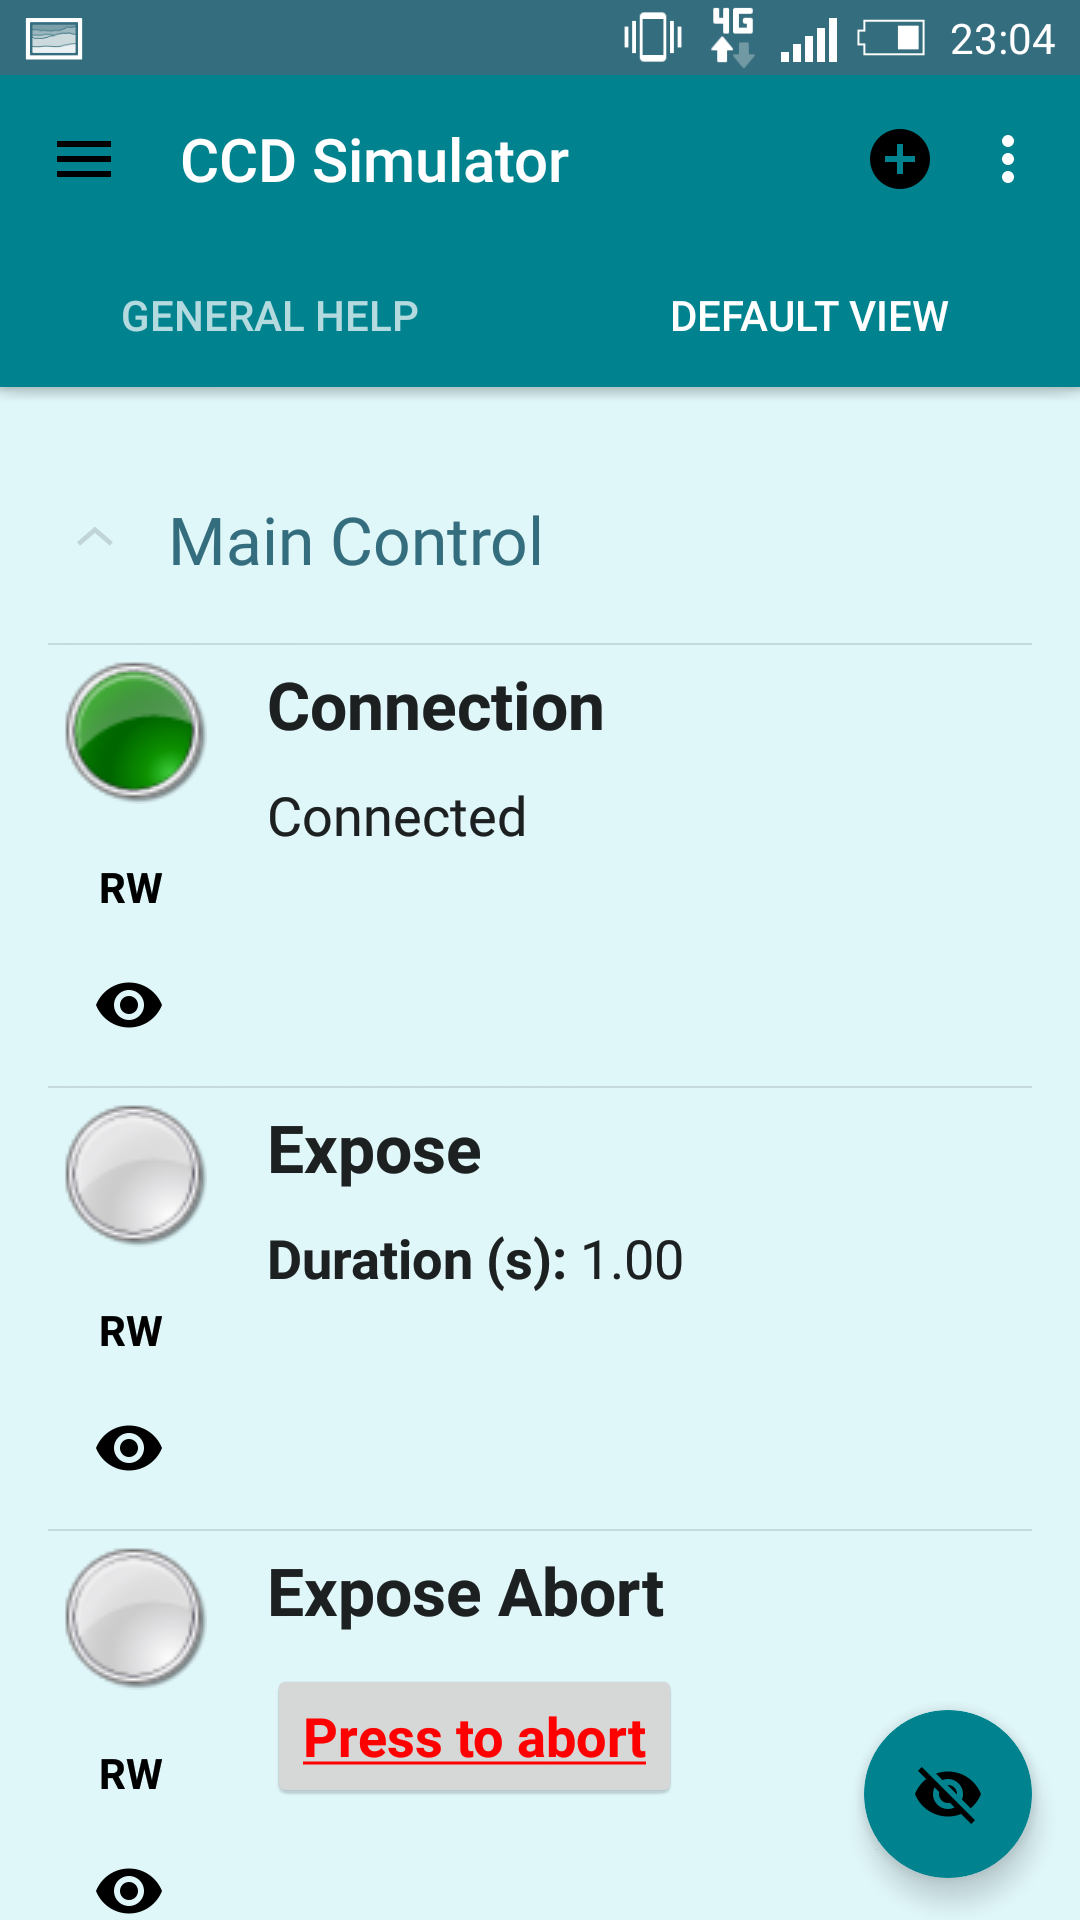
\includegraphics[width=0.3\textwidth]{../images/captura10.png}
  \caption{Vista de las propiedades connection y abort}
  \label{fig:connect_abort}
  \end{center}
\end{figure}

\newpage
\subsection{Dispositivos}
Al igual que con las propiedades, el software está diseñado para facilitar el diseño de nuevas clases para tener vistas especiales para algún dispositivo.

\bigskip
En el caso de las propiedades, se establecían prioridades para poder elegir de entre todas las posibilidades, cual iba a ser la interfaz de la propiedad concreta. En el caso de los dispositivos tenemos una interfaz de usuario por defecto, que lista las propiedades en una lista expandible. Pero se pueden añadir tantas como se deseen, pudiendo pasar de una a otra ya que se irían añadiendo al panel tabulado de la interfaz de usuario principal de la aplicación.

Para poder crear nuevas vistas para un dispositivo se ha diseñado la clase abstracta \texttt{DeviceView}.

\begin{lstlisting}[language=Java,caption={Clase abstracta DeviceView},label={lst:device_view}]
public abstract class DeviceView extends Fragment {

    static Device device;
    protected int layout;

    /**
     *  Check if this class can represent p
     *
     * @param dev Indi property
     * @return True/false if class can represent p
     */
    public abstract boolean handlesDevice (Device dev);

    public abstract String getName();

    @Override
    public abstract View onCreateView(LayoutInflater inflater, ViewGroup container, Bundle savedInstanceState);
}

\end{lstlisting}


\bigskip
Para poder crear una nueva vista de dispositivo debemos:

\begin{itemize}
  \item Crear una clase que herede de \texttt{deviceView}.
  \item Crear un archivo \textit{XML} con la definición de la interfaz de usuario.
  \item Añadir un objeto de la clase a la lista de clases manejadoras de dispositivos.
\end{itemize}


Como podemos ver en el fragmento de código \ref{lst:device_view}, tenemos dos atributos que son el dispositivo que vamos a manejar, y la referencia de \textbf{Android} al recurso donde se encuentra el archivo \textit{XML} con la definición de la vista. Además debemos implementar las siguientes funciones:


\begin{itemize}
  \item \texttt{handlesDevice}:
  Esta función recibe un dispositivo y debe comprobar si puede manejarlo o no devolviendo un valor booleano.

  \item \texttt{getName}:
  Esta función debe devolver el nombre que se desea que aparezca en la parte superior de la vista (vista tabulada).

  \item \texttt{onCreateView}:
  La clase abstracta hereda de \texttt{Fragment} y por ello esta función debe ser implementada, ya que se llamará cuando se llame a la clase para pintar la interfaz de usuario\cite{ALCA}. En ella deberemos crear la vista y realizar todas las inicializaciones que queramos.

\end{itemize}

\bigskip
Al igual que ocurría con las propiedades, debemos crear una vista definiéndola en un archivo \textit{XML} con los elementos visuales de \textbf{Android} que necesitemos.

\bigskip
Por último debemos agregar un objeto de nuestra clase a la lista de manejadores de dispositivos, como se ve en el fragmento de código \ref{lst:device_uis} llamando al método de la clase \texttt{Config} \texttt{addDeviceView(nuevo manejador)}

\begin{lstlisting}[language=Java,caption={Lista de objetos manejadores de dispositivos},label={lst:device_uis}]
private void setDeviceViews() {
    Config.addDeviceView(new DeviceMeteoView());
}

\end{lstlisting}

\bigskip
\section{Implementación}

Para un proyecto de desarrollo de software, las fases de análisis y diseño son claves para realizar la implementación. Uno de los objetivos del un proyecto fin de grado es demostrar la adquisición de competencias para realizar un correcto análisis de requisitos y un diseño exhaustivo. Estas fases previas realizadas correctamente aseguran una implementación más rápida. Por ello, la fase de implementación ha consistido en llevar a cabo todos los diagramas y especificaciones descritas en el diseño.

\bigskip
El código de la aplicación esta publicado bajo una licencia de \textbf{Software Libre} y puede ser consultada en \url{https://github.com/torresj/indi-android-ui}.

\bigskip
Para la implementación de este software, se ha usado el entorno de desarrollo \textbf{Android Studio} (Figura \ref{fig:android_studio}). Este entorno es el recomendado por \textb{Android} para realizar aplicaciones móviles.

\begin{figure}[!ht]
  \begin{center}
    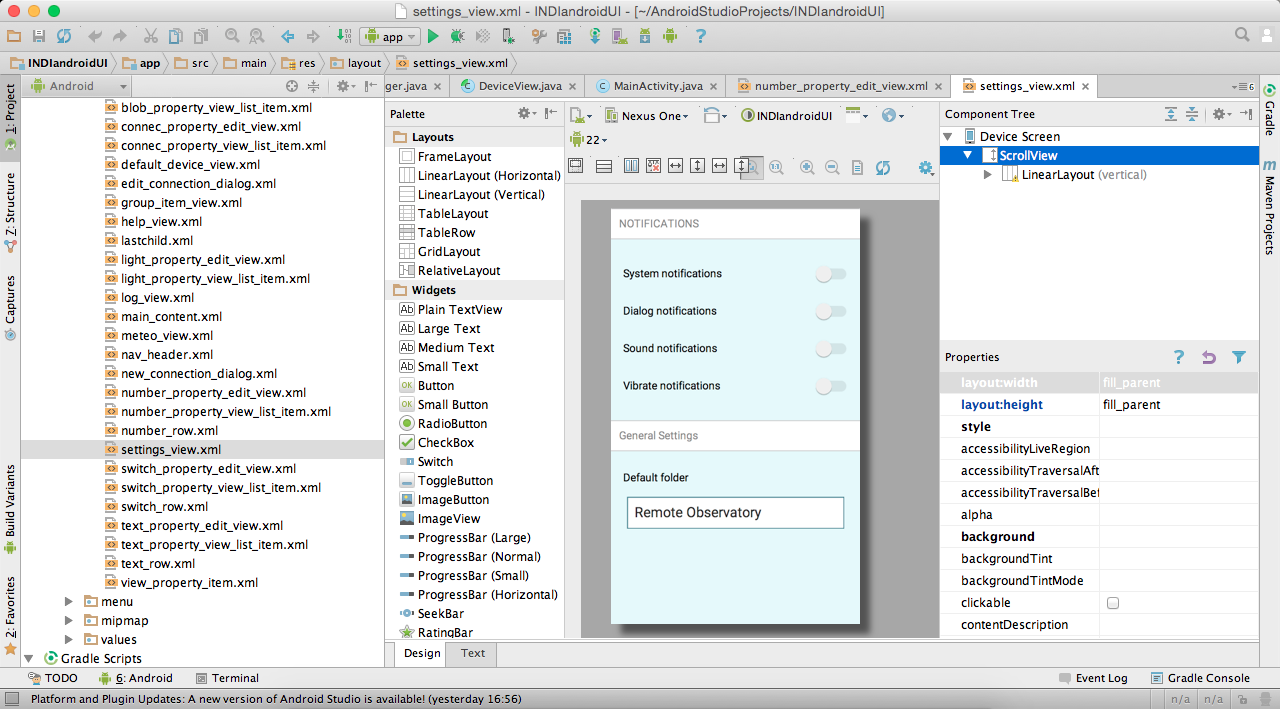
\includegraphics[width=1\textwidth]{../images/android_studio.png}
    \caption{Android Studio}
    \label{fig:android_studio}
  \end{center}
\end{figure}

\bigskip
También se ha usado para el desarrollo el procesador de textos \textbf{Sublime text}.

\bigskip
Para el control de versiones y publicación del código se ha utilizado \textbf{github} y la herramienta en linea \texttt{git} para poder subir los cambios desde un terminal.